\documentclass{../CNTeXBookTemplate/NanCNBook}

%\includeonly{}

\title{\hei\chuhao{Caffe\cite{jia2014caffe}解析}}
\author{nannanmath}

\begin{document}

\maketitle{}
\thispagestyle{empty}

\frontmatter
\pagestyle{plain}
\chapter*{前{\quad}言}
学习Caffe\footnote{http://caffe.berkeleyvision.org/}的设计与实现的细节,从而更好的实现机器学习相关的研究。

% \pagenumbering{roman}
\tableofcontents
\listoffigures
\listoftables

%\pagenumbering{arabic}
\mainmatter
\pagestyle{fancy}

\part{Caffe的依赖与结构}
% Chapter: C/C++编程基础
% Path: include/chp_c_basic/
\chapter{C/C++编程基础}
Caffe代码使用C/C++语言编写,了解一些C/C++语言的特性是读懂Caffe代码的前提。本章将根据实际情况,对Caffe中所使用的一些C/C++语言特性做简要介绍。
% Section X.1
\section{函数}
% Section X.1.1
\subsection{内联函数}\label{c/func/inline}
在C/C++中,内联函数是在定义时加入inline关键字的函数,这种函数在被调用时会在调用点别编译器展开,从而减少函数间调用的开销。但是在现代编译器中,这种展开操作将通过编译器自身进行判断和优化。
% Section X.1.2
\subsection{显式构造函数\cite{explicit-constructor}}\label{c/func/explicit}
在C++中, 带有一个参数的构造函数一般可以承担两个角色:一方面它是一个构造器;另一方面它也是一个默认且隐含的类型转换操作符,具体如下代码所示:
\begin{minted}{c++}
class String {
  String (const char* p); // 用C风格的字符串p作为初始化值
  //…
}
String s1 = "hello"; // 隐式转换,等价于String s1 = String("hello")
\end{minted}
但是有的时候可能会不需要这种隐式转换,如下:
\begin{minted}{c++}
class String {
  String (int n); // 本意是预先分配n个字节给字符串
  String (const char* p); // 用C风格的字符串p作为初始化值
  //…
}
// 下面两种写法比较正常:
String s2 (10);   // 显式调用,分配10个字节的空字符串
String s3 = String (10); // 显式调用,分配10个字节的空字符串

// 下面两种写法就比较疑惑了:
String s4 = 10; // 隐式转换,分配10个字节的空字符串
String s5 = 'a'; // 隐式转换,分配int('a')个字节的空字符串
\end{minted}
s4 和s5 分别把一个int型和char型隐式转换成了分配若干字节的空字符串,容易令人误解。
为了避免这种错误的发生,我们可以声明显示的转换,使用explicit 关键字:
\begin{minted}{c++}
class String {
  explicit String (int n); // 本意是预先分配n个字节给字符串
  String (const char* p); // 用C风格的字符串p作为初始化值
  //…
}
\end{minted}
加上explicit,就抑制了String (int n)的隐式转换,下面两种写法仍然正确:
\begin{minted}{c++}
String s2 (10);   // 分配10个字节的空字符串
String s3 = String (10); // 分配10个字节的空字符串
\end{minted}
下面两种写法就不允许了:
\begin{minted}{c++}
String s4 = 10; // 编译不通过,不允许隐式的转换
String s5 = 'a'; // 编译不通过,不允许隐式的转换
\end{minted}
因此,某些时候,explicit 可以有效得防止构造函数的隐式转换带来的错误或者误解。
% Section X.2
\section{宏}
% Section X.2.1
\subsection{do\{...\}while(0)}\label{c/macro/dowhile}
当我们定义的宏中有多条语句要顺序执行时,在使用这样的宏时就要多加注意,例如下边的情况:
\begin{minted}{c++}
#define DOSOMETHING()\
  foo1();\
  foo2();
\end{minted}
通过宏的方式定义了一个名称为DOSOMETHING()函数,在使用这个宏时,如果通过如下方法:
\begin{minted}{c++}
if(a>0)
  DOSOMETHING();
\end{minted}
因为宏在预处理的时候会直接被展开,实际上的代码是这个样子的:
\begin{minted}{c++}
if(a>0)
  foo1();
foo2();
\end{minted}
这就会导致程序逻辑错误,因为无论a是否大于0,foo2()都会被执行。如果使用\{\}将宏中的语句包裹起来,那么宏的定义就是:
\begin{minted}{c++}
#define DOSOMETHING() \
{ \
  foo1(); \
  foo2(); \
}
\end{minted}
通过使用上面的调用方式使用该宏,就会得到如下展开:
\begin{minted}{c++}
if(a>0)
{
  foo1();
  foo2();
};
\end{minted}
这就会出现编译错误。在实际编程中,为了避免这几种错误,通常使用如下方法定义一个包含多条顺序执行语句的宏。
\begin{minted}{c++}
#define DOSOMETHING() \
  do { \
    foo1();\
    foo2();\
  } while(0)
\end{minted}
这种方式的宏定义在Caffe源代码中会经常见到,同时也十分值得我们在编程时借鉴使用。
% Section X.2.2
\subsection{带有\#和\#\#的宏}\label{c/macro/sharp}
简单的说,\#\#把前后两个符号连接起来,而\#则返回一个与后边符号一至的字符串。同时,对于使用\#的宏,在展开时与普通宏页存在差异,下面通过一个例子进行说明。
\begin{minted}{c++}
#define f(a,b) a##b
#define d(a) #a
#define s(a) d(a) 
\end{minted}
如上方式定义三个宏,并通过如下方法进行调用:
\begin{minted}{c++}
void main( void ) {
  puts(d(f(a,b)));
  puts(s(f(a,b)));
} 
\end{minted}
输出的结果分别为:
\begin{minted}{c++}
f(a,b)
ab
\end{minted}
对于宏d(a),由于是以\#开头,因此在语句puts(d(f(a,b)))中,其参数直接替换,不进行展开。而对于宏s(a),由于不是以\#开头,因此在语句puts(s(f(a,b)))中,其参数要先进行展开,然后再进行替换。
% Section X.3
\section{指针}
% Section X.3.1
\subsection{const指针}\label{c/ptr/constptr}
const指针是指:指针本身为const,也就是说指针指向的数据可以被修改但是指针本身存储的地址不能改变。如下所示:
\begin{minted}{c++}
  int a = 3;
  int b = 4;
  int* const ptr = &a; //定义一个const指针,必须被初始化

  *ptr = 4; // 可以成功执行
  ptr = &b; // 编译错误
\end{minted}
% Section X.3.2
\subsection{指向const的指针}\label{c/ptr/ptr2const}
指向const的指针是指:指针指向一个const修饰的变量类型,因此指针指向的内存里的变量值不可以被修改,但是指针本身存储的地址值可以被修改。如下所示:
\begin{minted}{c++}
  int a = 3;
  int b = 4;
  const int* ptr; //定义一个const指针,可以不初始化

  *ptr = 4; // 编译错误
  ptr = &b; // 可以成功编译
\end{minted}
% Section X.4
\section{类型转换}
C++提供了四个转换运算符:
const\_cast <type-id> (expression)、static\_cast <type-id> (expression)、reinterpret\_cast <type-id> (expression)和dynamic\_cast <type-id> (expression)。
% Section X.4.1
\subsection{static\_cast <type-id> (expression)}\label{c/type/static}
该运算符把expression转换为type-id类型,转换过程在编译时完成,因此没有运行时类型检查来保证转换的安全性。static\_cast不能转换掉expression的const、volatile、或者\_\_unaligned属性。在基类与派生类之间指针或引用的转换中,该运算符进行上行转换(把派生类的指针或引用转换成基类表示)是安全的;进行下行转换(把基类指针或引用转换成派生类表示)时,由于没有动态类型检查,所以是不安全的。
% Section X.4.2
\subsection{dynamic\_cast <type-id> (expression)}
该运算符通常在基类和派生类之间转换时使用,转换过程发生在运行时,因此具有类型检查的功能,比static\_cast更安全。在基类与派生类之间指针或引用的转换,该运算符进行上行转换(把派生类的指针或引用转换成基类表示)是安全的;进行下行转换(把基类指针或引用转换成派生类表示)时,如果基类指针或者引用确实指向一个派生类对象,这个运算符会传回适当转型过的指针;如果基类指针或者引用没有指向一个派生类对象,这个运算符会传回空指针。具体例子如下:
\begin{minted}{c++}
#include <iostream>  
using namespace std;  
class A {  
 public:  virtual void show() {  
   std::cout<<"A::show()"<<endl;  
 }  
};  
class B : public A {  
 public:
  virtual void show() {   
    std::cout<<"B::show()"<<endl;  
  }  
};  

int main() {  
  A* pa=new A();  
  B* pb=new B();  
  cout<<"-------- 1 ----------"<<endl;  
  static_cast<A*>(pb)->show(); //print:"B::show()"  
  cout<<"-------- 2 ----------"<<endl;  
  dynamic_cast<A*>(pb)->show();//also print:"B::show()"  
  cout<<"-------- 3 ----------"<<endl;  
  static_cast<B*>(pa)->show(); //print:"A::show()"   
  cout<<"-------- 4 ----------"<<endl;  
  //dynamic_cast<B*>(pa)->show(); //此处会出现异常  
  if((pb = dynamic_cast<B*>(pa))) {  
    pb->show();  
  } else {  
    cout << "dynamic cast fail" << endl;  
  }  
}  
\end{minted}
% Section X.4.3
\subsection{const\_cast <type-id> (expression)}
该运算符用来转换掉表达式的const性质的。例子如下:
\begin{minted}{c++}
const char m = 't';  
const char *cm = &m;  
char *n = const_cast<char*>(cm);  
*n = 'a';  
cout << *n << endl; 
\end{minted}
% Section X.4.4
\subsection{reinterpret\_cast <type-id> (expression)}
该运算符是强制类型转换符,用来处理无关类型的转换,通常为操作数的位模式提供较低层次的重新解释,但是并没有进行二进制的转换。它可以用在任意的指针之间的转换,引用之间的转换,指针和足够大的int型之间的转换,整数到指针的转换。例子如下:

\begin{minted}{c++}
int *pi;  
char *pc = reinterpret_cast<char*>(pi);
\end{minted}
下面给出一个实际应用的例子,基于地址的哈希编码:
\begin{minted}{c++}
unsigned short Hash( void *p ) {  
  unsigned int val = reinterpret_cast<unsigned int>( p );  
  return ( unsigned short )( val ^ (val >> 16));
}

using namespace std;  
int main() {  
  int a[20];  
  for ( int i = 0; i < 20; i++ )  
    cout << Hash( a + i ) << endl;  
}  
\end{minted}
\section{C/C++标准库}
类型:
std::vector<>
std::pair<>
方法:
std::partial\_sort()
std::cout << std::fixed << std::setprecision(4)

\section{常用头文件介绍}
\begin{itemize}
\item <climits> \\
  其中定义了常用数据类型的最小和最大值。
\item <cmath> \\
  数学库
\item <fstream> \\
  文件流
\item <iostream> \\
  输入输出流
\item <map> \\
  映射
\item <set> \\
  集合
\item <sstream> \\
  流
\item <string> \\
  字符串
\item <utility> \\
  pair
\item <vector> \\
  向量
\item <algorithm> \\
  
\end{itemize}


% Chapter: CUDA编程基础
% Path: include/chp_cuda_basic/
\chapter{CUDA编程基础}
现代机器学习中大量使用GPU设备来节省算法的运行时间,Caffe的一个重要特性就是对GPU的支持。但是,基于GPU的编程又是一个庞大的学习任务,因此本章将对GPU编程做简要介绍,目的是能够理解Caffe代码中关于GPU的使用。

% Section X.1
\section{内存管理}
% Section X.1.1
\subsection{分配内存}\label{cuda/mem/alloc}
\subsubsection{cudaMalloc()}
\begin{cnfrmfunc}
   \item{\kai{原型}}\\
      ​cudaError\_t cudaMalloc ( void** devPtr, size\_t size )
   \item{\kai{参数}}\\
     devPtr - 指向分配内存的指针\\
     size - 要分配的内存的大小
   \item{\kai{返回值}}\\
     cudaSuccess, cudaErrorMemoryAllocation
\end{cnfrmfunc}
  对于GPU设备端(device)内存的分配,常用的函数有cudaMalloc(void** ptr, int size),该函数返回一个cudaError\_t类型的值。该函数在GPU显存上分配size个字节的空间,并在保存于主机端(host)的ptr所指向的内存中写入一个device端的地址(注意ptr指向的内存只能存放指针变量),该地址指向显存。
\subsubsection{cudaMallocHost()}
\begin{cnfrmfunc}
   \item{\kai{原型}}\\
     cudaError\_t cudaMallocHost 	(void** ptr, size\_t size) 	
   \item{\kai{参数}}\\
     ptr - 指向分配内存的指针\\
     size - 要分配的内存的大小
   \item{\kai{返回值}}\\
     cudaSuccess, cudaErrorMemoryAllocation
\end{cnfrmfunc}     
然而在host端分配内存时,可以使用cudaMallocHost(void** ptr, int size)或者cuda函数,该函数与常用的malloc()函数的区别是分配的内存为页锁定内存(Pinned Memory)。由于GPU知道内存的物理地址,因此可以使用直接内存访问技术(Direct Memory Access)在host和device之间复制数据,无需CPU的参与,可以提高效率。然而由于分配的内存为页锁定,因此无法使用虚拟内存技术,有耗尽主机内存的风险。
% Section X.1.2
\subsection{内存初始化}\label{cuda/mem/init}
\subsubsection{cudaMemset()}
\begin{cnfrmfunc}
   \item{\kai{原型}}\\
     cudaError\_t cudaMemset ( void* devPtr, int  value, size\_t count )
   \item{\kai{参数}}\\
     devPtr - 要设置的设备内存首地址
     value - 要设置的整型值
     count - 要设置的字节数
   \item{\kai{返回值}}\\
     cudaSuccess, cudaErrorInvalidValue, cudaErrorInvalidDevicePointer
\end{cnfrmfunc}
初始化设备端内存,将设备端指定内存设置为统一数值。
\subsubsection{cudaMemcpy()}
\begin{cnfrmfunc}
   \item{\kai{原型}}\\
      ​cudaError\_t cudaMemcpy ( void* dst, const void* src, size\_t count, cudaMemcpyKind kind )
   \item{\kai{参数}}\\
     dst - 拷贝目的地址\\
     src - 拷贝源地址\\
     count - 拷贝字节数\\
     kind - 拷贝类型
   \item{\kai{返回值}}\\
     cudaSuccess, cudaErrorInvalidValue, cudaErrorInvalidDevicePointer, cudaErrorInvalidMemcpyDirection
\end{cnfrmfunc}
该函数实现主机与设备之间的内存拷贝功能,其中kind参数的可选类型为:
\begin{cntable}{kind参数类型}{tab:cuda/mem/init/kind}
  \begin{tabular}{|c|l|}
    \hline
    类型 & 功能 \\ \hline
    cudaMemcpyHostToHost & 主机端与主机端内存拷贝 \\ \hline
    cudaMemcpyHostToDevice & 住居端向设备端内存拷贝 \\ \hline
    cudaMemcpyDeviceToHost & 设备端向主机端内存拷贝 \\ \hline
    cudaMemcpyDeviceToDevice & 设备端与设备端内存拷贝 \\ \hline
    cudaMemcpyDefault & 使用统一虚拟地址空间 \\ \hline
  \end{tabular}
\end{cntable}
\subsubsection{cudaMemcpyAsync()}
\begin{cnfrmfunc}
   \item{\kai{原型}}\\
     ​cudaError\_t cudaMemcpyAsync ( void* dst, const void* src, size\_t count, cudaMemcpyKind kind, cudaStream\_t stream = 0 )
   \item{\kai{参数}}\\
     dst - 拷贝目的地址\\
     src - 拷贝源地址\\
     count - 拷贝字节数\\
     kind - 拷贝类型\\
     stream - CUDA流号
   \item{\kai{返回值}}\\
     cudaSuccess, cudaErrorInvalidValue, cudaErrorInvalidDevicePointer, cudaErrorInvalidMemcpyDirection
\end{cnfrmfunc}
该函数可以异步执行一个内存拷贝操作,所以当函数调用返回时无法保证拷贝操作已经完成。这里需要重点介绍的是该函数的最后一个参数,流。流是为了实现并行执行两个或多个不同任务(也称做并发执行)而引入的概念。CUDA中的流是一个GPU操作队列,被添加到流中的操作会按照指定的顺序被执行。对于一个支持设备重叠功能的GPU,硬件在处理内存复制和核函数执行时分别采用不同的引擎:内存复制引擎和核函数执行引擎,能够在执行一个核函数的同时执行内存的复制操作,因此可以使用多个流来实现这种计算与数据传输的重叠。通过stream参数可以将内存复制操作添加到指定流中。
% Section X.1.3
\subsection{内存释放}\label{cuda/mem/free}
\subsubsection{cudaFreeHost()}
\begin{cnfrmfunc}
   \item{\kai{原型}}\\
    cudaError\_t cudaFreeHost (void* ptr)
   \item{\kai{参数}}\\
     ptr 指向待释放内存的指针
   \item{\kai{返回值}}\\
     cudaSuccess, cudaErrorInitializationError
\end{cnfrmfunc}
释放由cudaMallocHost()或者cudaHostAlloc()函数分配的页锁定内存。
\subsubsection{cudaFree()}
\begin{cnfrmfunc}
   \item{\kai{原型}}\\
      ​cudaError\_t cudaFree ( void* devPtr )
   \item{\kai{参数}}\\
     devptr 指向待释放内存的指针
   \item{\kai{返回值}}\\
     cudaSuccess, cudaErrorInvalidDevicePointer, cudaErrorInitializationError
\end{cnfrmfunc}
释放由cudaMalloc()或cudaMallocPitch()分配的内存。
% Section 2
\section{错误管理}\label{cuda/err}
\subsubsection{cudaGetErrorString()}
\begin{cnfrmfunc}
\item{\kai{原型}}\\
const char* cudaGetErrorString (cudaError\_t error) 
\item{\kai{参数}}\\
error - CUDA函数返回错误代码\\
\item{\kai{返回值}}\\
const char*
\end{cnfrmfunc}
该函数将CUDA函数返回的错误代码转换为字符串信息。

% Section 3
\section{设备设置}\label{cuda/basic/device}
\subsubsection{cudaGetDevice()}
\begin{cnfrmfunc}
\item{\kai{原型}}\\
cudaError\_t cudaGetDevice ( int* device ) 
\item{\kai{参数}}\\
device - 存储正在运行的设备号\\
\item{\kai{返回值}}\\
cudaSuccess
\end{cnfrmfunc}
获得当前主机线程所执行设备代码所在的设备号。
\subsubsection{cudaSetDevice()}
\begin{cnfrmfunc}
\item{\kai{原型}}\\
cudaError\_t cudaSetDevice ( in device ) 
\item{\kai{参数}}\\
device - 特定设备号\\
\item{\kai{返回值}}\\
cudaSuccess, cudaErrorInvalidDevice, cudaErrorDeviceAlreadyInUse
\end{cnfrmfunc}
将特定设备号的设备指定为当前设备。



% Chapter: Caffe的依赖库
% Path: include/chp_deps_libs/
\chapter{Caffe的依赖库}
Caffe代码的实现依赖了大量第三方功能库(特别是使用了多个Google公司的开源库),在“站在巨人的肩膀上”的同时,也为Caffe代码的学习带来一定困难。本章将对这些依赖库的功能和使用做简要介绍。
% Section X.1
\section{准标准库Boost}
Boost库定义在namespace boost中。
% Section X.1.1
\subsection{智能指针}\label{deps/boost/ptr}
\subsubsection{scoped\_ptr<T>}
scoped\_ptr<T>是Boost中最简单的智能指针,当指针离开其作用域时候,释放相关资源。需要特别注意的一点是scoped\_ptr<T>不能共享指针的所有权也不能转移所有权,因此该指针不能作为函数返回值使用。
\begin{minted}{c++}
class test { 
 public: 
  void print() { 
    cout << "test print now" <<endl; 
  } 
};

int _tmain(int argc, _TCHAR* argv[]) { 
  boost::scoped_ptr<test> x(new test); 
  x->print(); 
  return 0; 
}
\end{minted}
\subsubsection{shared\_ptr<T>}
shared\_ptr<T>是Boost智能指针中最常使用的指针,该指针中包含一个引用计数器,当类型为T的对象的引用数量为0时,该对象所在的堆内存会被自动释放。这里要注意的是该指针不能指向一块动态增长的内存(可以使用share\_array<T>代替)。
\begin{minted}{c++}
class test { 
 public: 
  void print() { 
    cout << "test print now" <<endl; 
  } 
};

int _tmain(int argc, _TCHAR* argv[]) { 
  boost::shared_ptr<test> ptr_1(new test); 
  ptr_1->print();//引用计数为1
  boost::shared_ptr<test> ptr_2 = ptr_1; 
  ptr_2->print();//引用计数为2
  ptr_1->print();//引用计数还是为2
  return 0; 
}
\end{minted}
\subsubsection{weak\_ptr<T>}
weak\_ptr是一个弱指针,它可以共享一个share\_ptr的内存,但是无论是构造还是析构一个weak\_ptr 都不会影响引用计数器。
\subsubsection{intrusive\_ptr<T>}
intrusive\_ptr和share\_ptr功能一样,但比share\_ptr效率高,不过intrusive\_ptr要求类型T本身维护一个引用计数器。
\subsubsection{scoped\_array<T> 和 shared\_array<T>}
shared\_ptr和scoped\_ptr不能用于数组的内存,所以shared\_array和scoped\_array可以作为他们的代替品。但是,这里还是建议使用std::vector<shared\_ptr>。
\begin{minted}{c++}
int _tmain(int argc, _TCHAR* argv[]) { 
  const int size = 10; 
  boost::shared_array<test> a(new test[]);
  for (int i = 0; i < size; ++i) 
    a[i].print();
  return 0; 
}
\end{minted}

% Section X.2
\section{日志功能glog库}\label{deps/glog}
% Section X.3
\section{程序参数处理gflags库}\label{deps/gflags}
% Section X.4
\section{单元测试gtest库}
% Section X.5
\section{结构化protobuffer库}\label{deps/protobuf}
全称为Protocol Buffers,是一种结构化数据存储格式,可以对存储数据进行序列化和反序列化,可用于网络中的结构化数据传输。在Caffe中,protobuffer主要用来存储和管理支持网络运行的各种相关参数,它可以将参数以对象的形式序列化后存储于二进制文件中,然后通过反序列化对其进行读取。
% Section X.5.1
\subsection{使用介绍}
% Section X.5.2
\subsection{Caffe中Protobuffer的结构}

% Section X.6
\section{图像处理opencv库}
类型:
cv::Size
cv::Scalar
方法:
cv::merge()
cv::mean()
cv::cvtColor()
cv::resize()
cv::Mat的convertTo()
cv::subtract()
cv::splite()
cv::imread()
cv::Mat(height, width, type, data)
cv::Mat(cv::Size, type, cv::Scalar)
% Section X.7
\section{代数运算BLAS}
BLAS全称Basic Linear Algebra Subprograms,是线性代数运算中所需算法的集合,其中包括诸如向量加法、向量乘法、矩阵乘法等。BLAS最早起源于Fortran,其中定义的函数接口后来被其他代数运算库做为标准接口使用,这些运算库包括:ATLAS、Intel Math Kernel Library (MKL)和OpenBLAS等。在NVIDIA公司的CUDA SDK中也包括了一个叫做cuBLAS的BLAS实现,主要应用于该公司的GPU产品。
% Section X.7.1
\subsection{CPU端的BLAS}\label{deps/blas/cpu}
\subsubsection{cblas\_*axpy()}
\begin{cnfrmfunc}
   \item{\kai{原型}}\\ 
     void cblas\_saxpy(const int n, const float a, const float* x, const int incx float* y, int incy) \\
     void cblas\_daxpy(const int n, const double a, const double* x, const int incx double* y, int incy)
   \item{\kai{参数}}\\
     n - x和y中元素个数\\
     a - 尺度系数\\
     x - 数组x首地址\\
     incx - x的计算间隔\\
     y - 数组y首地址\\
     incy- y的计算间隔
   \item{\kai{返回值}}\\
     float或double
   \item{\kai{描述}}\\
     $y\coloneqq a*x+y$
\end{cnfrmfunc}
\subsubsection{cblas\_*asum()}
\begin{cnfrmfunc}
   \item{\kai{原型}}\\ 
     float cblas\_sasum (const int n, const float *x, const int incx)\\
     double cblas\_dasum (const int n, const double *x, const int incx)
   \item{\kai{参数}}\\
     n - x和y中元素个数\\
     x - 数组x首地址\\
     incx - x的计算间隔
   \item{\kai{返回值}}\\
     float或者double
   \item{\kai{描述}}\\
     $res\coloneqq \sum\limits_{i}^{n}x[i]$
\end{cnfrmfunc}
\subsubsection{cblas\_*dot()}
\begin{cnfrmfunc}
   \item{\kai{原型}}\\ 
     float cblas\_sdot (const int n, const float *x, const int incx, const float *y, const int incy)\\
     double cblas\_ddot (const int n, const float *x, const int incx, const float *y, const int incy)
   \item{\kai{参数}}\\
     n - x和y中元素个数\\
     x - 数组x首地址\\
     incx - x的计算间隔\\
     y - 数组y的首地址\\
     incy - y的计算间隔
   \item{\kai{返回值}}\\
     float或者double
   \item{\kai{描述}}\\
     $res\coloneqq \sum\limits_{i}^{n}x[i]*y[i]$
\end{cnfrmfunc}
\subsubsection{cblas\_*scal()}
\begin{cnfrmfunc}
  \item{\kai{原型}}\\
    void cblas\_sscal (const int n, const float a, float *x, const int incx)\\
    void cblas\_dscal (const int n, const double a, double *x, const int incx)
   \item{\kai{参数}}\\
     n - x和y中元素个数\\
     a - 系数\\
     x - 数组x首地址\\
     incx - x的计算间隔\\
   \item{\kai{返回值}}\\
     空值
   \item{\kai{描述}}\\
     $res\coloneqq a * x[i]$
\end{cnfrmfunc}   
   
 % Section X.7.2
\subsection{GPU端的BLAS}\label{deps/blas/gpu}
\subsubsection{cublas*axpy()}
\begin{cnfrmfunc}
   \item{\kai{原型}}\\ 
     cublasStatus\_t cublasSaxpy(cublasHandle\_t handle, int n,
                           const float           *alpha,
                           const float           *x, int incx,
                           float                 *y, int incy)\\
     cublasStatus\_t cublasDaxpy(cublasHandle\_t handle, int n,
                           const double          *alpha,
                           const double          *x, int incx,
                           double                *y, int incy)
   \item{\kai{参数}}\\
     handle - cuBLAS库的句柄\\                      
     n - x和y中元素个数\\
     alpha - 尺度系数\\
     x - 数组x首地址\\
     incx - x的计算间隔\\
     y - 数组y首地址\\
     incy- y的计算间隔
   \item{\kai{返回值}}\\
     cublasStatus\_t
   \item{\kai{描述}}\\
     $y\coloneqq a*x+y$
\end{cnfrmfunc}
\subsubsection{cublas*asum()}
\begin{cnfrmfunc}
   \item{\kai{原型}}\\ 
     cublasStatus\_t  cublasSasum(cublasHandle\_t handle, int n,
                                 const float *x, int incx, float  *result)\\
     cublasStatus\_t  cublasDasum(cublasHandle\_t handle, int n,
                                 const double *x, int incx, double *result)
   \item{\kai{参数}}\\
     handle - cuBLAS库的句柄\\                      
     n - x中元素个数\\
     x - 数组x首地址\\
     incx - x的计算间隔\\
     result - 保存计算的结果
   \item{\kai{返回值}}\\
     cublasStatus\_t
   \item{\kai{描述}}\\
     $result\coloneqq \sum\limits_{i}^{n}x[i]$
\end{cnfrmfunc}
\subsubsection{cublas*dot()}
\begin{cnfrmfunc}
   \item{\kai{原型}}\\ 
     cublasStatus\_t cublasSdot (cublasHandle\_t handle, int n,
                                const float *x, int incx,
                                const float *y, int incy,
                                float *result)\\
     cublasStatus\_t cublasDdot (cublasHandle\_t handle, int n,
                                const double *x, int incx,
                                const double *y, int incy,
                                double *result)
   \item{\kai{参数}}\\
     handle - cuBLAS库的句柄\\                      
     n - x中元素个数\\
     x - 数组x首地址\\
     incx - x的计算间隔\\
     y - 数组y首地址\\
     incy - y的计算间隔\\
     result - 保存计算的结果
   \item{\kai{返回值}}\\
     cublasStatus\_t
   \item{\kai{描述}}\\
     $result\coloneqq \sum\limits_{i}^{n}x[i]*y[i]$
\end{cnfrmfunc}
\subsubsection{cublas*scal()}
\begin{cnfrmfunc}
   \item{\kai{原型}}\\ 
     cublasStatus\_t  cublasSscal(cublasHandle\_t handle, int n,
                                 const float *alpha,
                                 float *x, int incx)\\
     cublasStatus\_t  cublasDscal(cublasHandle\_t handle, int n,
                                 const double *alpha,
                                 double *x, int incx)
   \item{\kai{参数}}\\
     handle - cuBLAS库的句柄\\                      
     n - x中元素个数\\
     alpha - 系数\\
     x - 数组x首地址\\
     incx - x的计算间隔\\
   \item{\kai{返回值}}\\
     cublasStatus\_t
   \item{\kai{描述}}\\
     $x[i]\coloneqq alpha * x[i]$
\end{cnfrmfunc}
   




\chapter{Caffe的层次}

\part{Caffe的外部调用}

\chapter{从examples开始} % include/chp_from_examples/
% section 1
% title: 图像分类classification.cpp
\section{图像分类classification.cpp}
该例子程序实现了通过Caffe进行图像分类的功能,在使用中需要借助OpenCV的帮助以实现图像的读写操作。下面来学习具体的实现过程。
\begin{minted}{c++}
#include <caffe/caffe.hpp>
#ifdef USE_OPENCV
#include <opencv2/core/core.hpp>
#include <opencv2/highgui/highgui.hpp>
#include <opencv2/imgproc/imgproc.hpp>
#endif  // USE_OPENCV
#include <algorithm>
#include <iosfwd>
#include <memory>
#include <string>
#include <utility>
#include <vector>
\end{minted}
在Caffe中,所用的核心功能都已经编译为一个动态链接库,使用该库需要首先将Caffe的头文件caffe/caffe.hpp包含进来。接着可以看到一个包含OpenCV的与编译宏,然后是一些使用到的头文件。
\begin{minted}{c++}
#ifdenf USE_OPENCV
...
#else
int main(int argc, char** argv) {
  LOG(FATAL) << "This example requires OpenCV; compile with USE_OPENCV.";
}
#endif  // USE_OPENCV
\end{minted}
其实这个程序的整个代码都被写在一个预编译宏中,用来强调对OpenCV的依赖。
在保证可以满足OpenCV依赖之后,程序使用caffe命名空间和string域,并定义一个pair类型变量,用来存贮分类的结果和得分。
\begin{minted}{c++}
using namespace caffe;  // NOLINT(build/namespaces)
using std::string;

/* Pair (label, confidence) representing a prediction. */
typedef std::pair<string, float> Prediction;
\end{minted}

\subsection{Classifier类的声明}
Classifier类是分类功能的核心部分,也是整个程序中唯一的类,其声明部分代码如下:
\begin{minted}{c++}
class Classifier {
 public:
  Classifier(const string& model_file,
             const string& trained_file,
             const string& mean_file,
             const string& label_file);

  std::vector<Prediction> Classify(const cv::Mat& img, int N = 5);

 private:
  void SetMean(const string& mean_file);

  std::vector<float> Predict(const cv::Mat& img);

  void WrapInputLayer(std::vector<cv::Mat>* input_channels);

  void Preprocess(const cv::Mat& img,
                  std::vector<cv::Mat>* input_channels);

 private:
  shared_ptr<Net<float> > net_;
  cv::Size input_geometry_;
  int num_channels_;
  cv::Mat mean_;
  std::vector<string> labels_;
};
\end{minted}

从声明中可也看出,该类的构造函数需要输入4个参数,如表\ref{chp-examples-classification-cpp1}所示,这些文件也是Caffe学习中常用到的一些文件,他们是Caffe能够正常运行的重要部分,也是机器学习中的用来调整参数的重要文件。
\begin{cntable}{参数}{chp-examples-classification-cpp1}
  \begin{tabular}{|c|l|}
    \hline
    model\_file & 网络模型定义文件 \\ \hline
    trained\_file & 训练好的模型文件 \\ \hline
    mean\_fiel & 数据均值文件 \\ \hline
    label\_file & 保存标记的文件 \\
    \hline
  \end{tabular}
\end{cntable}

\subsection{构造函数}
Classifier类的定义已经在前文做了简要说明,下边对该类进行拆分,并对其中的成员做一一介绍。

\begin{minted}{c++}
#ifdef CPU_ONLY
  Caffe::set_mode(Caffe::CPU);
#else
  Caffe::set_mode(Caffe::GPU);
#endif
\end{minted}
在构造函数中以预编译宏的方式,通过调用Caffe内建方法set\_mode()来控制程序运行是否使用GPU。
\begin{minted}{c++}
  /* Load the network. */
  net_.reset(new Net<float>(model_file, TEST));
  net_->CopyTrainedLayersFrom(trained_file);

  CHECK_EQ(net_->num_inputs(), 1) << "Network should have exactly one input.";
  CHECK_EQ(net_->num_outputs(), 1) << "Network should have exactly one output.";

  Blob<float>* input_layer = net_->input_blobs()[0];
  num_channels_ = input_layer->channels();
  CHECK(num_channels_ == 3 || num_channels_ == 1)
    << "Input layer should have 1 or 3 channels.";
  input_geometry_ = cv::Size(input_layer->width(), input_layer->height());
\end{minted}
对Classifier类中的私有成员指针型变量shared\_ptr<Net<float> > net\_进行构造,该变量指的是Caffe中的神经网络结构(由Caffe的Net类管理),在类中使用了Boost库的Shared\_ptr智能指针。在Net类的构造中需要指定model\_file参数和运行类型为TEST模式(因为不需要进行网络训练),然后使用reset()方法将net\_指针指向一个新构造的Net对象。获得网络结构后,使用Net类的CopyTrainedLayersFrom(trained\_file)方法将训练好的模型加载(拷贝)到该网络,然后使用gtest库的CHECK\_EQ()方法对输入和输出层数进行检查,如果二者不相等,那么程序运行就会被终止并输出错误说明。


为了获得输入图像的相关信息,定义一个Blob<float>类型的指针变量input\_layer并指向网络的第一个输入blob,(通过Net类的input\_blobs()方法可以获得输入层的所有blob地址所组成的数组的指针,然后取数组中第一个地址中的值,也就是指向第一个blob的指针,这里要注意的是一个blob对象可以存储多副图像)。接着就可以通过input\_layer变量获得输入图像的通道数input\_layer->channels(),并将该值存入Classifier类的成员变量num\_channels\_中,然后检查通道数是否为3或者1。对于图像的尺度,可以使用OpenCV库的Size方法,构造一个Size对象用来存储。

\begin{minted}{c++}
/* Load the binaryproto mean file. */
  SetMean(mean_file);
\end{minted}
使用Calssifier类的Setmean()方法加载均值文件,用来将输入图像数据进行中心化。这个方法在后文会详细讲解。

\begin{minted}{c++}
/* Load labels. */
  std::ifstream labels(label_file.c_str());
  CHECK(labels) << "Unable to open labels file " << label_file;
  string line;
  while (std::getline(labels, line))
    labels_.push_back(string(line));

  Blob<float>* output_layer = net_->output_blobs()[0];
  CHECK_EQ(labels_.size(), output_layer->channels())
    << "Number of labels is different from the output layer dimension.";
\end{minted}
定义ifstream流对象labels来获取标签文件,使用gtest的CHECK检查文件是否正差打开。使用getline()函数获得标签文件中的每一行并存入预先定义的line字符串中,然后将其按行压入Classifier类的成员变量labels\_中,该变量定义为一个元素为字符串的向量std::vector<string> labels\_。


定义一个Blob型的指针变量output\_layer指向网络的输出net\_->output\_blobs()[0],然后检查label的个数是否与输出blob的通道数相同,该值事实上就是分类的类别数。

\subsection{预测结果排序}
Caffe对一副图像的类别进行预测的结果是该图像属于不同类别的概率值(也可以看作一个打分),数值越大则该图像隶属于对应类别的可能性越高。因此在预测结束后需要对每个类别的隶属分数进行一个排序,将对应分数最高的类别定为最终的分类结果。


\begin{minted}{c++}
static bool PairCompare(const std::pair<float, int>& lhs,
                        const std::pair<float, int>& rhs) {
  return lhs.first > rhs.first;
}

/* Return the indices of the top N values of vector v. */
static std::vector<int> Argmax(const std::vector<float>& v, int N) {
  std::vector<std::pair<float, int> > pairs;
  for (size_t i = 0; i < v.size(); ++i)
    pairs.push_back(std::make_pair(v[i], i));
  std::partial_sort(pairs.begin(), pairs.begin() + N, pairs.end(), PairCompare);

  std::vector<int> result;
  for (int i = 0; i < N; ++i)
    result.push_back(pairs[i].second);
  return result;
}
\end{minted}
程序中使用的排序方法间接用到了C/C++的标准库函数partial\_sort(),该函数可以按照一个预定义的方法对std::vector中的对象元素进行排序,该预定义方法的返回值是一个bool值。在本程序中,预定义的方法即为PairCompare(),该方法按照pair结构中第一个值的大小顺序对两个pair对象进行排序。方法Argmax()首先使用std::make\_pair()构造pair对象(pair中的第一个值类别对应的float型得分分数,第二个值为int型类别序号),然后使用partial\_sort()对vector中的pair对象进行排序,排序后的vector中的前N个值对应由PairCompare()方法得到的最大的N个pair,最后构造一个vector<int>型变量result用来存储排序后pair中的类别序号部分,并返回该result。在这里,方法PairCompare()和Argmax()都是静态方法,因此不属于Classifier类。

\subsection{对图像进行预测}
\begin{minted}{c++}
/* Return the top N predictions. */
std::vector<Prediction> Classifier::Classify(const cv::Mat& img, int N) {
  std::vector<float> output = Predict(img);

  N = std::min<int>(labels_.size(), N);
  std::vector<int> maxN = Argmax(output, N);
  std::vector<Prediction> predictions;
  for (int i = 0; i < N; ++i) {
    int idx = maxN[i];
    predictions.push_back(std::make_pair(labels_[idx], output[idx]));
  }

  return predictions;
}
\end{minted}
Classifier的Classify()函数将对一副由OpenCV读取的图像进行类别预测,并返回一个vector<Prediction>类型的预测结果。Classify()函数内部将调用另一个成员函数Predict()以得到图像在每个类别上的得分,然后通过Argmax()函数对得分进行排序并返回前N个最大得分所对应的序号,根据序号和得分构造一个vector<Prediction> predictions类型的变量,用来存储前N个标签名称和对应得分值。注意,Prediction类型已经在程序文件开始处进行了定义。

\subsection{均值文件的读取}
对于均值文件的读取和格式转换,在Classifier类的成员函数SetMean()中主要分为三个步骤:
\begin{minted}{c++}
BlobProto blob_proto;
  ReadProtoFromBinaryFileOrDie(mean_file.c_str(), &blob_proto);
\end{minted}
首先是定义一个BlobProto型变量blob\_proto,然后调用ReadProtoFromBinaryFileOrDie()函数读取均值文件并将数据存入blob\_proto变量中。

\begin{minted}{c++}
/* Convert from BlobProto to Blob<float> */
  Blob<float> mean_blob;
  mean_blob.FromProto(blob_proto);
  CHECK_EQ(mean_blob.channels(), num_channels_)
    << "Number of channels of mean file doesn't match input layer.";
\end{minted}
第二步是使用Blob类型的FromProto函数,将上步读取的BlobProto类型数据转换为Blob类型数据,并存入mean\_blob中。

\begin{minted}{c++}
/* The format of the mean file is planar 32-bit float BGR or grayscale. */
  std::vector<cv::Mat> channels;
  float* data = mean_blob.mutable_cpu_data();
  for (int i = 0; i < num_channels_; ++i) {
    /* Extract an individual channel. */
    cv::Mat channel(mean_blob.height(), mean_blob.width(), CV_32FC1, data);
    channels.push_back(channel);
    data += mean_blob.height() * mean_blob.width();
\end{minted}
第三步也是完成一个类型转换功能,将存入mean\_blob变量中的Blob类型数据转换为OpenCV中的Mat类型数据,这里直接使用了Mat类型的构造函数,通过传入Mat的长度、宽度和数据指针的方式对每个通道的数据进行存储转换,流程如图\ref{classification_cpp_binaryproto_to_mat}。注意这里用到了Blob类型的数据指针函数mutable\_cpu\_data(),具体细节将在后续章节介绍。
\begin{cnfigure}{binaryproto文件读取流程}{classification_cpp_binaryproto_to_mat}
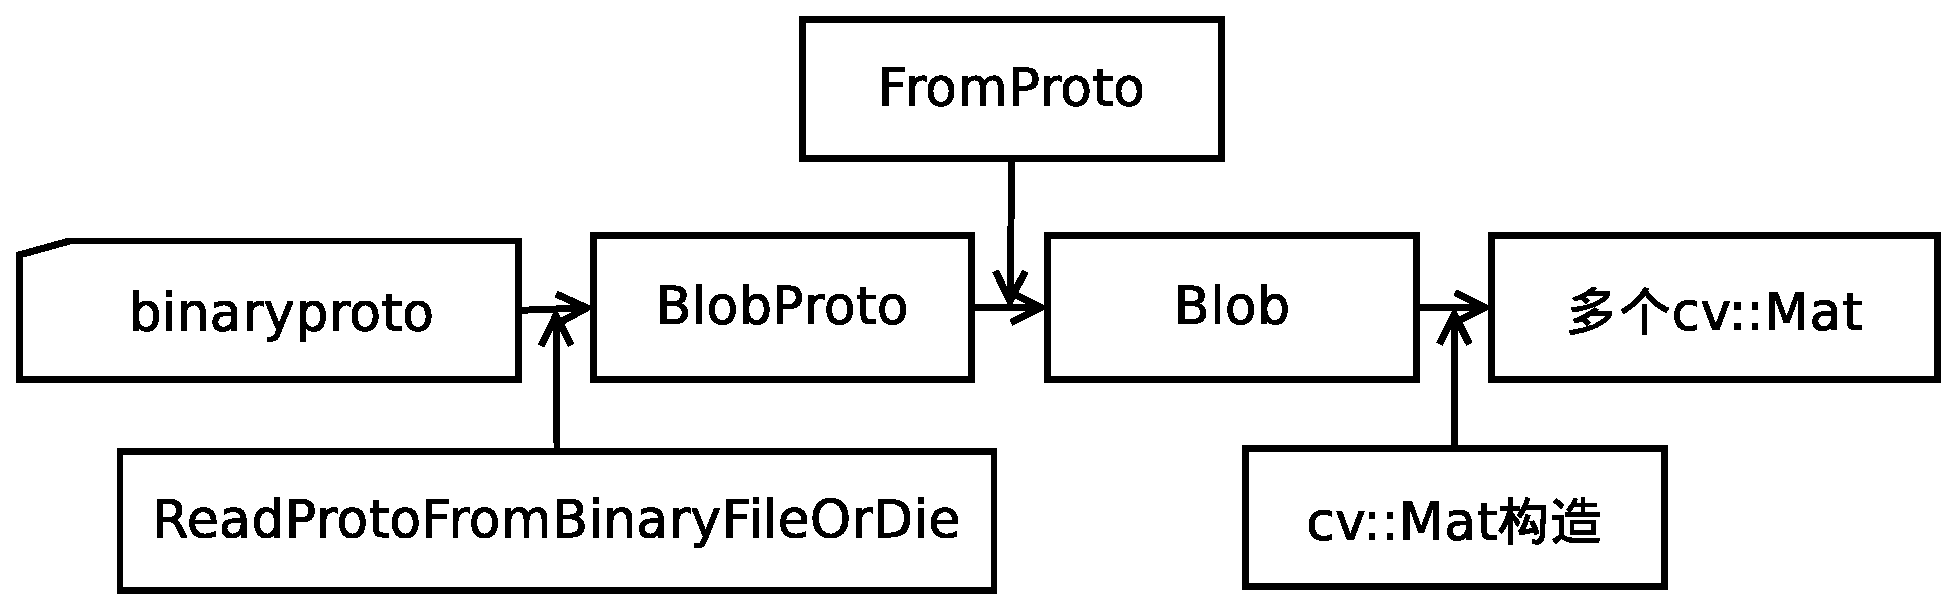
\includegraphics[height=5cm ,width=15cm,angle=0]{include/chp_from_examples/figures/classification_cpp_binaryproto_to_mat.eps}
\end{cnfigure}

完成以上三步的数据读取之后,均值数据已经分通道存储为OpenCV的Mat类型,存储变量为std::vector<cv::Mat> channels。接下来要利用OpenCV求取真正的均值并生成一个多通道Mat格式文件。
\begin{minted}{c++}
/* Merge the separate channels into a single image. */
  cv::Mat mean;
  cv::merge(channels, mean);
\end{minted}
cv::merge()方法将多个Mat融合为一个多通道Mat,存储在mean变量中。
\begin{minted}{c++}
/* Compute the global mean pixel value and create a mean image
   * filled with this value. */
  cv::Scalar channel_mean = cv::mean(mean);
  mean_ = cv::Mat(input_geometry_, mean.type(), channel_mean);
}
\end{minted}
cv::mean()方法对mean中的每个通道求取均值,返回的结果存储在cv::Scalar类型变量channel\_mean中,并使用该变量和cv::Mat的构造函数生成最终需要的均值Mat,结果存储到Classifier类的成员变量mean\_中。

\subsection{预测函数}
Classifier类的成员函数Predict()可以完成对一副图像的预测,输出每个类别的得分。
\begin{minted}{c++}
std::vector<float> Classifier::Predict(const cv::Mat& img) {
  Blob<float>* input_layer = net_->input_blobs()[0];
  input_layer->Reshape(1, num_channels_,
                       input_geometry_.height, input_geometry_.width);
  /* Forward dimension change to all layers. */
  net_->Reshape();

  std::vector<cv::Mat> input_channels;
  WrapInputLayer(&input_channels);

  Preprocess(img, &input_channels);

  net_->Forward();

  /* Copy the output layer to a std::vector */
  Blob<float>* output_layer = net_->output_blobs()[0];
  const float* begin = output_layer->cpu_data();
  const float* end = begin + output_layer->channels();
  return std::vector<float>(begin, end);
}
\end{minted}
首先获得网络输入层Blob对象的指针Blob<float>* input\_layer,通过该指针对输入层的Blob对象进行一次Reshape操作input\_layer->Reshape(1, num\_channels\_, input\_geometry\_.height, input\_geometry\_.width),注意,由于输入图像只有一副,因此第一个参数是1。然后执行net\_->Reshape对整个网络进行一次Reshape。接下来要将图像数据送入网络,这里首先使用WrapInputLayer(\&input\_channels)对网络的输入部分构造一个wrap(见后文介绍),目标是简化输入过程,然后调用Preprocess()方法,对输入图像进行预处理,以满足网络正常运行的要求,最后调用net\_->Forward()进行一次前向过程,得到网络输出。使用Blob<float>* output\_layer = net\_->output\_blobs()[0]获得输出Blob对象指针,然后根据通道数分别得到数据部分的开头和结尾处指针,最后根据两处指针的位置构造一个vector<float>(begin, end)对象并返回,其中存储的便是对应每个类别的得分值。

\subsection{对输入Blob进行包裹}
此处是整个程序代码的一个亮点,在使用Caffe时很值得借鉴。
\begin{minted}{c++}
void Classifier::WrapInputLayer(std::vector<cv::Mat>* input_channels) {
  Blob<float>* input_layer = net_->input_blobs()[0];

  int width = input_layer->width();
  int height = input_layer->height();
  float* input_data = input_layer->mutable_cpu_data();
  for (int i = 0; i < input_layer->channels(); ++i) {
    cv::Mat channel(height, width, CV_32FC1, input_data);
    input_channels->push_back(channel);
    input_data += width * height;
  }
}
\end{minted}
首先获得网络输入层的Blob对象指针,并获得该对象中的数据指针存入input\_data。对于每一个数据通道,构造cv::Mat对象(每个Mat对象的数据通过input\_data指针获得),依次将对象压入函数参数vector<cv::Mat>* input\_channels中,如图\ref{classification_cpp_wrap}这样就在网络的输入Blob和vector<cv::Mat>之间构建了一座桥梁,在使用中,只要对input\_channels指向的数据进行修改,就等价于对网络输入层的Blob对象的数据部分进行了修改。这种思路很值得借鉴。
\begin{cnfigure}{Wrap示意图}{classification_cpp_wrap}
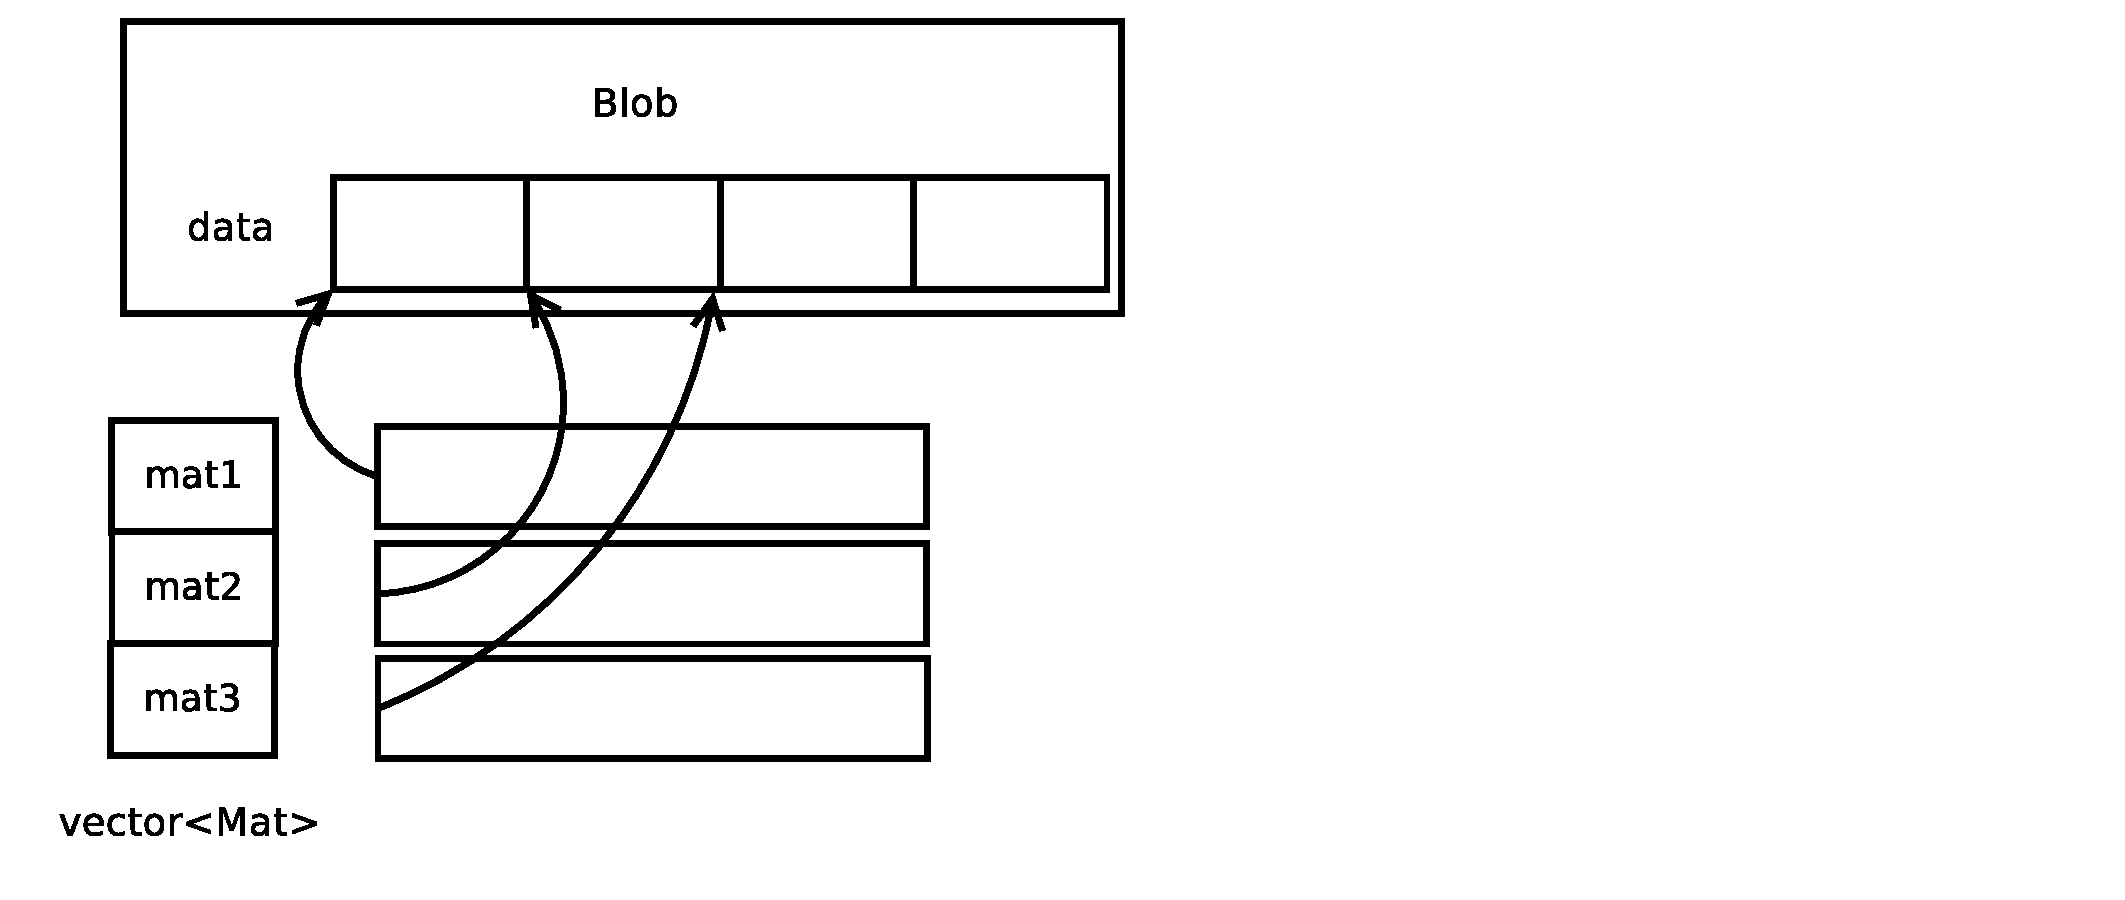
\includegraphics[height=6cm ,width=14cm,angle=0]{include/chp_from_examples/figures/classification_cpp_wrap.eps}
\end{cnfigure}


\subsection{图像预处理}
Classifier类的Preprocess()成员函数完成对输入图像的预处理,使得处理后的图像能够满足网络运行的需要。这里所有的处理操作都是通过OpenCV库来完成的。
\begin{minted}{c++}
/* Convert the input image to the input image format of the network. */
cv::Mat sample;
if (img.channels() == 3 && num_channels_ == 1)
  cv::cvtColor(img, sample, cv::COLOR_BGR2GRAY);
else if (img.channels() == 4 && num_channels_ == 1)
  cv::cvtColor(img, sample, cv::COLOR_BGRA2GRAY);
else if (img.channels() == 4 && num_channels_ == 3)
  cv::cvtColor(img, sample, cv::COLOR_BGRA2BGR);
else if (img.channels() == 1 && num_channels_ == 3)
  cv::cvtColor(img, sample, cv::COLOR_GRAY2BGR);
else
  sample = img;
\end{minted}
首先对图像的通道数进行转换,其中num\_channels\_是由读入的网络定义文件确定的,因此其目的是将图像通道数转换为与网络定义输入文件通道数一至。这里使用了cv::cvtColor()方法

\begin{minted}{c++}
cv::Mat sample_resized;
if (sample.size() != input_geometry_)
  cv::resize(sample, sample_resized, input_geometry_);
else
  sample_resized = sample;
\end{minted}
input\_geometry\_是cv::Size类型,其中存储了网络结构定义的输入图像的长度和宽度,如果真实图像与所需不符,那么就进行转换。这里使用了cv::resize()方法。

\begin{minted}{c++}
cv::Mat sample_float;
if (num_channels_ == 3)
  sample_resized.convertTo(sample_float, CV_32FC3);
else
  sample_resized.convertTo(sample_float, CV_32FC1);
\end{minted}
将图像数据从int型转换为float型。这里使用了cv::Mat类的convertTo()方法。

\begin{minted}{c++}
cv::Mat sample_normalized;
cv::subtract(sample_float, mean_, sample_normalized);
\end{minted}
对图像进行中心化,使用cv::subtract()方法,减去均值mean\_。

\begin{minted}{c++}
cv::split(sample_normalized, *input_channels);
\end{minted}
通过cv::splite()方法,将cv::Mat型数据按通道分别存储到vector<cv::Mat>* input\_channels中,由于这里经过Wrap处理,因此input\_channels已经与输入层的Blob对象绑定,该操作也就直接将图像数据传入到了网络输入层,全部流程如图\ref{classification_cpp_image_transform}。
\begin{cnfigure}{图像变换流程}{classification_cpp_image_transform}
  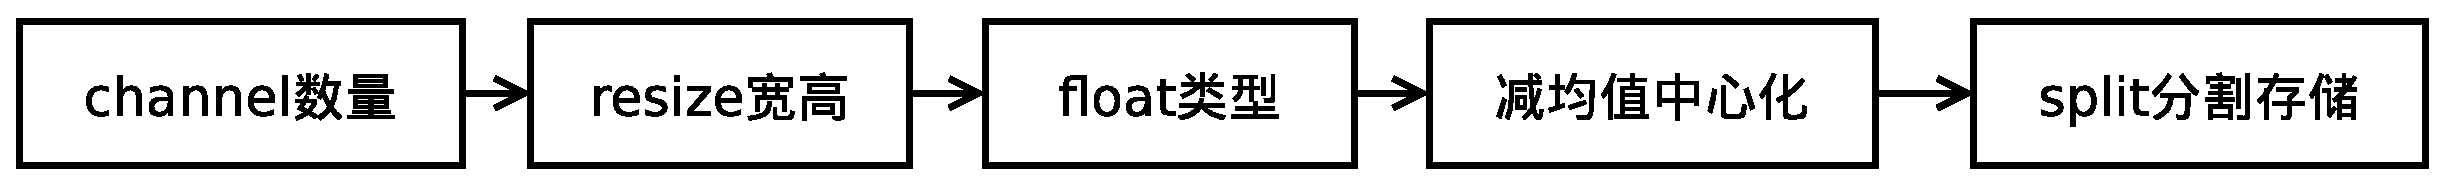
\includegraphics[height=1cm ,width=15cm,angle=0]{include/chp_from_examples/figures/classification_cpp_image_transform.eps}
\end{cnfigure}

\begin{minted}{c++}
CHECK(reinterpret_cast<float*>(input_channels->at(0).data)
        == net_->input_blobs()[0]->cpu_data())
    << "Input channels are not wrapping the input layer of the network.";
\end{minted}
在最后阶段,检查包裹过程是否成功,这里使用了C/C++标准库的reinterpret\_cast<>()方法进行类型转换,判断input\_channels中第一个Mat的数据首地址是否与网络输入层中Blob对象的数据首地址一至。


\subsection{主函数}
\begin{minted}{c++}
if (argc != 6) {
  std::cerr << "Usage: " << argv[0]
            << " deploy.prototxt network.caffemodel"
            << " mean.binaryproto labels.txt img.jpg" << std::endl;
  return 1;
}
\end{minted}
主函数中,首先检查输入参数是否为6个,这里要注意第一个参数永远为是程序本身。

\begin{minted}{c++}
::google::InitGoogleLogging(argv[0]);
\end{minted}
由于程序要用到glog库,因此在这里进行一个初始化,初始化所用到的参数为程序名本身,也就是argv[0]。

\begin{minted}{c++}
string model_file   = argv[1];
string trained_file = argv[2];
string mean_file    = argv[3];
string label_file   = argv[4];
Classifier classifier(model_file, trained_file, mean_file, label_file);
\end{minted}
处理每一个传入的参数,并使用这些参数初始化一个Classifier对象。

\begin{minted}{c++}
string file = argv[5];

std::cout << "---------- Prediction for "
          << file << " ----------" << std::endl;

cv::Mat img = cv::imread(file, -1);
CHECK(!img.empty()) << "Unable to decode image " << file;
std::vector<Prediction> predictions = classifier.Classify(img);
\end{minted}
最后一个参数(第5个参数)是要进行预测的图像文件路径。使用OpenCV的cv::imread()函数读取该图像文件,然后调用Classifier类对象的Classify()方法对图像类别进行预测,返回前N个(程序默认为前5个)得分最大的类别结果和分数。

\begin{minted}{c++}
for (size_t i = 0; i < predictions.size(); ++i) {
  Prediction p = predictions[i];
  std::cout << std::fixed << std::setprecision(4) << p.second << " - \""
            << p.first << "\"" << std::endl;
  }
\end{minted}
打印返回的结果,并在输出时设定格式和精度std::cout << std::fixed << std::setprecision(4)。


\chapter{常用工具tools}
在Caffe代码的tools目录下包含了诸多作为tools的工具软件代码,他们通过对Caffe核心功能的调用实现各种外层的逻辑应用。
\section{计算图像均值compute\_image\_mean.cpp}

\section{图像写入数据库convert\_query.cpp}

\section{训练与测试caffe.cpp}
caffe.cpp实现了一个网络的训练与测试功能,是Caffe中最常用的程序。该程序中包含很多技巧,其中一些很值得在软件开发中借鉴使用。


首先判断是否启用python\_layer:
\begin{minted}{c++}
#ifdef WITH_PYTHON_LAYER
#include "boost/python.hpp"
namespace bp = boost::python;
#endif
\end{minted}
通过Makefile判断是否启用python\_layer,如果启用则包含Boost库的boost::python库,实现python调用C++功能。


使用gflags进行参数设置:
\begin{minted}{c++}
DEFINE_string(gpu, "",
    "Optional; run in GPU mode on given device IDs separated by ','."
    "Use '-gpu all' to run on all available GPUs. The effective training "
    "batch size is multiplied by the number of devices.");
DEFINE_string(solver, "",
    "The solver definition protocol buffer text file.");
DEFINE_string(model, "",
    "The model definition protocol buffer text file.");
DEFINE_string(snapshot, "",
    "Optional; the snapshot solver state to resume training.");
DEFINE_string(weights, "",
    "Optional; the pretrained weights to initialize finetuning, "
    "separated by ','. Cannot be set simultaneously with snapshot.");
DEFINE_int32(iterations, 50,
    "The number of iterations to run.");
DEFINE_string(sigint_effect, "stop",
             "Optional; action to take when a SIGINT signal is received: "
              "snapshot, stop or none.");
DEFINE_string(sighup_effect, "snapshot",
             "Optional; action to take when a SIGHUP signal is received: "
             "snapshot, stop or none.");
\end{minted}
其中包含的参数有:gpu,solver,model,snapshot,weights,iteration,sigint\_effect和sighup\_effect。主要功能见表\ref{tab:参数说明}:
\begin{table}[h]
  \setlength{\abovecaptionskip}{-5pt}
  \caption{参数说明}
  \centering
  \begin{tabular}{|c|l|}
    \hline
    gpu & 是否使用GPU运行 \\ \hline
    solver & solver文件路径 \\ \hline
    model & 模型路径 \\ \hline
    snapshot & 参数文件保存路径 \\ \hline
    weights & 参数文件路径 \\ \hline
    iterations & 最大迭代次数 \\ \hline
    sigint\_effect & 不知道 \\ \hline
    sighup\_effect & 不知道 \\
    \hline
  \end{tabular}
  \label{tab:参数说明}
\end{table}
                    
\section{特征提取extract\_feature.cpp}

\section{网络微调finetune\_net.cpp}

\part{Caffe的内部实现}
% Chapter: 数学运算及辅助函数
% Path: include/chp_math_funcs/
\chapter{数学运算及辅助函数}
Caffe将底层的数学运算和一些辅助函数专门进行了分离,统一保存在名为math\_functions.hpp、math\_functions.cpp和math\_functions.cu的文件中,其中math\_functions.cu是GPU上运行的函数实现。
% Section X.1
\section{数学运算函数}
% Section X.1.1
\subsection{CPU函数}
% Section X.1.2
\subsection{GPU函数}
% Section X.2
\section{存储操作}
% Section X.2.1
\subsection{内存初始化}\label{math/mem/init}
\subsubsection{caffe\_memset()}
\begin{cnfrmfunc}
   \item{\kai{原型}}\\
     inline void caffe\_memset(const size\_t N, const int alpha, void* X)
   \item{\kai{参数}}\\
     N - 字节数\\
     alpha - 初始值\\
     X - 内存首地址
   \item{\kai{返回值}}\\
     空值
\end{cnfrmfunc}
该函数内部将调用memset()函数进行内存赋值。
\subsubsection{caffe\_gpu\_memset()}
\begin{cnfrmfunc}
   \item{\kai{原型}}\\
     inline void caffe\_gpu\_memset(const size\_t N, const int alpha, void* X)
   \item{\kai{参数}}\\
     N - 字节数\\
     alpha - 初始值\\
     X - 内存首地址
   \item{\kai{返回值}}\\
     空值
\end{cnfrmfunc}
该函数内部将调用cudaMemset()函数进行内存赋值(参考~\ref{cuda/mem/init})。
% Section X.2.2
\subsection{内存拷贝}\label{math/mem/cpy}
\subsubsection{caffe\_gpu\_memcpy()}
\begin{cnfrmfunc}
   \item{\kai{原型}}\\
     void caffe\_gpu\_memcpy(const size\_t N, const void* X, void* Y)
   \item{\kai{参数}}\\
     N - 拷贝字节数\\
     X - 待拷贝内存首地址(设备端)\\
     Y - 拷贝目的地址(主机端)
   \item{\kai{返回值}}\\
     空值
\end{cnfrmfunc}
该函数将数据从设备端拷贝至主机端。函数具体实现如下:
\begin{minted}{c++}
void caffe_gpu_memcpy(const size_t N, const void* X, void* Y) {
  if (X != Y) {
    CUDA_CHECK(cudaMemcpy(Y, X, N, cudaMemcpyDefault));  // NOLINT(caffe/alt_fn)
  }
}
\end{minted}
通过调用cudaMemcpy()函数实现(参考~\ref{cuda/mem/init}),注意这里的拷贝目的地址Y与使用统一地址空间的设备之间可以分享,函数最后一个参数设置为cudaMemcpyDefault。

% Chapter: CUDA辅助宏
% Path: include/chp_cuda_macro/
\chapter{CUDA辅助宏}
Caffe中定义了一些列的宏和函数对CUDA相关操作做了一定的处理,这些宏和函数一头文件的形式保存在device\_alternate.hpp中,下边将对其做简要介绍。
% Section X.1
\section{GPU模式相关}\label{cudamacro/gpumode}
\subsubsection{NO\_GPU宏}
该宏一般在检测到程序没有启用GPU模式时被调用,宏内部使用了glog库,显示一段字符串标明没有使用GPU模式。
\begin{minted}{c++}
#define NO_GPU LOG(FATAL) << "Cannot use GPU in CPU-only Caffe: check mode."
\end{minted}
% Section X.2
\section{CUDA返回错误处理}\label{cudamacro/err}
\subsubsection{CUDA\_CHECK()宏}
检测CUDA函数的返回值是否出错,通过glog库的CHECK宏判断返回值是否为error,如果为error则调用cudaGetErrorString()(参考\ref{cuda/err})函数输出错误信息。
\begin{minted}{c++}
#define CUDA_CHECK(condition) \
  /* Code block avoids redefinition of cudaError_t error */ \
  do { \
    cudaError_t error = condition; \
    CHECK_EQ(error, cudaSuccess) << " " << cudaGetErrorString(error); \
  } while (0)
\end{minted}
\subsubsection{CUBLAS\_CHECK()宏}
检测CUDA函数的返回值是否出错,通过glog库的CHECK宏判断返回值是否为error,如果为error则调用cublasGetErrorString()(参考\ref{common/err/cublas})函数输出错误信息。
\begin{minted}{c++}
#define CUBLAS_CHECK(condition) \
  do { \
    cublasStatus_t status = condition; \
    CHECK_EQ(status, CUBLAS_STATUS_SUCCESS) << " " \
      << caffe::cublasGetErrorString(status); \
  } while (0)
\end{minted}
\subsubsection{CURAND\_CHECK()宏}
检测CUDA函数的返回值是否出错,通过glog库的CHECK宏判断返回值是否为error,如果为error则调用curandGetErrorString()(参考\ref{common/err/curand})函数输出错误信息。
\begin{minted}{c++}
#define CURAND_CHECK(condition) \
  do { \
    curandStatus_t status = condition; \
    CHECK_EQ(status, CURAND_STATUS_SUCCESS) << " " \
      << caffe::curandGetErrorString(status); \
  } while (0)
\end{minted}

% Section X.3
\section{CUDA线程相关}


% Chapter: common文件
% Path: include/chp_common_file/
\chapter{common文件}
在Caffe源代码中有两个文件,名称分别为common.hpp和common.cpp,这里统称为common文件。common文件中包含了一些Caffe中常使用的宏定义、全局初始化函数定义和Caffe类的定义,其中后两者都包含在caffe命名空间中。
% Section X.1
\section{常用的宏}
% Section X.1.1
\subsection{宏名转为字符串}
\begin{minted}{c++}
#define STRINGIFY(m) #m
#define AS_STRING(m) STRINGIFY(m)
\end{minted}
在使用时,如果m是一个宏的名字,那么AS\_STRING(m)将得到一个与该宏名一至的字符串。关于这类含有\#字符的宏的详细说明,请参考\ref{c/macro/sharp}。
% Section X.1.2
\subsection{修正gflags的一个问题}
\begin{minted}{c++}
#ifndef GFLAGS_GFLAGS_H_
namespace gflags = google;
#endif  // GFLAGS_GFLAGS_H_
\end{minted}
如代码注释部分所述,对于版本号为2.1的gflags库,其命名空间由原来的google被替换为gflags,因此Caffe通过检查是否存在宏定义GFLAGS\_GFLAGS\_H\_来判断当前gflags的版本,如果为2.1那么就对命名空间名称进行替换。
% Section X.1.3
\subsection{禁止对类对象进行拷贝和赋值操作}\label{common/macro/discpy}
\begin{minted}{c++}
#define DISABLE_COPY_AND_ASSIGN(classname) \
private:\
  classname(const classname&);\
  classname& operator=(const classname&)
\end{minted}
在c++编程中,在有些特殊情况下,往往希望禁止类对象的拷贝和赋值操作,最常见的方法是把对应类中的拷贝构造函数和赋值函数定义为私有类型,并且没有任何实现代码。以上定义的宏就是基于这个思路,使用时,只要在类的声明主体中加入该宏,并将参数改为类名即可。


% Chapter: Proto文件
% Path: include/chp_proto_file/
\chapter{Proto文件}
Caffe中的Proto文件用于描述Caffe运行所需的各项参数信息,文件名为caffe.proro。
\section{Blob相关}\label{proto/file/blob}
Proto文件中关于Blob部分主要描述数据存储成员对象和数据维度:
\begin{minted}{c++}
// Specifies the shape (dimensions) of a Blob.
message BlobShape {
  repeated int64 dim = 1 [packed = true];
}

message BlobProto {
  optional BlobShape shape = 7;
  repeated float data = 5 [packed = true];
  repeated float diff = 6 [packed = true];
  repeated double double_data = 8 [packed = true];
  repeated double double_diff = 9 [packed = true];

  // 4D dimensions -- deprecated.  Use "shape" instead.
  optional int32 num = 1 [default = 0];
  optional int32 channels = 2 [default = 0];
  optional int32 height = 3 [default = 0];
  optional int32 width = 4 [default = 0];
}

// The BlobProtoVector is simply a way to pass multiple blobproto instances
// around.
message BlobProtoVector {
  repeated BlobProto blobs = 1;
}
\end{minted}
在message BlobProto中已经放弃通过num、channels、height和width字段的方式来描述Blob对象中数据维度(但是目前仍然可用),而是使用一个新定义的message BlobShape来进行描述,同时该字段为optional类型。

% Chapter: 底层数据管理syncedmemory类
% Path: include/chp_syncedmem_cls/
\chapter{底层数据管理SyncedMemory类}
SyncedMemory类提供了数据的内存分配、释放以及在主机端(host)与设备端(device)之间的拷贝等功能,是Caffe基本数据存储类型(Blob类)的基础。
% section X.1
\section{内存分配与释放}
在SyncedMemory.hpp文件中首先定义了caffe命名空间中的两个关于内存分配和释放相关的函数:
\subsubsection{CaffeMallochost()}
\begin{cnfrmfunc}
   \item{\kai{原型}}\\
     inline void CaffeMallocHost(void** ptr, size\_t size, bool* use\_cuda)
   \item{\kai{参数}}\\
     ptr - 指向分配内存的指针\\
     use\_cuda - 是否要在GPU上分配内存数据
   \item{\kai{返回值}}\\
     空值
   \end{cnfrmfunc}
函数的具体实现代码:
\begin{minted}{c++}
inline void CaffeMallocHost(void** ptr, size_t size, bool* use_cuda) {
#ifndef CPU_ONLY
  if (Caffe::mode() == Caffe::GPU) {
    CUDA_CHECK(cudaMallocHost(ptr, size));
    *use_cuda = true;
    return;
  }
#endif
  *ptr = malloc(size);
  *use_cuda = false;
  CHECK(*ptr) << "host allocation of size " << size << " failed";
}
\end{minted}
函数CaffeMallocHost()用来对内存进行分配,如果在编译时没有指明只使用CPU模式,那么将调用cudaMallocHost()分配页锁定内存,详细叙述可以参考\ref{cuda/mem/alloc},然后通过宏CUDA\_CHECK()(参考~\ref{cudamacro/err})检查内存是否被成功分配。如果指明仅使用CPU模式,那么将调用常规的malloc()函数。
\subsubsection{CaffeFreehost()}
\begin{cnfrmfunc}
   \item{\kai{原型}}\\
     inline void CaffeFreeHost(void* ptr, bool use\_cuda)
   \item{\kai{参数}}\\
     ptr - 指向待释放内存的指针\\
     use\_cuda - GPU上是否由数据
   \item{\kai{返回值}}\\
     空值
   \end{cnfrmfunc}
函数的具体实现代码:
\begin{minted}{c++}
inline void CaffeFreeHost(void* ptr, bool use_cuda) {
#ifndef CPU_ONLY
  if (use_cuda) {
    CUDA_CHECK(cudaFreeHost(ptr));
    return;
  }
#endif
  free(ptr);
}  
\end{minted}
函数CaffeFreeHost()用来对分配的内存进行释放。由于分配的内存为页锁定内存,因此调用了cudaFreeHost()函数进行释放(参考~\ref{cuda/mem/free})。

% Section X.2
\section{Syncedmemory类的结构}
% Section X.2.1
\subsection{成员变量}
\begin{cntable}{成员变量}{syncedmem/cls/memvar}
  \begin{tabular}{|c|c|l|}
    \hline
    变量名 & 类型 & 功能 \\ \hline
    cpu\_ptr\_ & void* & 主机端数据指针 \\ \hline
    gpu\_ptr\_ & void* & 设备端数据指针 \\ \hline
    size\_ & size\_t &  数据大小 \\ \hline
    head\_ & Syncedhead & 说明数据所在位置,参考~表\ref{syncedmem/cls/syncedhead} \\ \hline
    own\_cpu\_data\_ & bool & 主机端指针指向的数据内存是否由该类分配 \\ \hline
    cpu\_malloc\_use\_cuda\_ & bool & 是否使用GPU,分配页锁定内存 \\ \hline
    own\_gpu\_data\_ & bool & 设备端指针指向的数据内存是否由该类分配\\ \hline
    gpu\_device\_ & int & 设备号 \\ \hline
  \end{tabular}
\end{cntable}
其中,size\_t类型在不同操作系统下代表不同长度的类型,在32位系统下,可以理解为unsigned int型,为32位长度;在64位系统像,可以理解为long unsigned int型,为64位长度。目的是为了方便移植。

Syncedhead是一个枚举类型,定义为enum SyncedHead \{ UNINITIALIZED, HEAD\_AT\_CPU, HEAD\_AT\_GPU, SYNCED \},其具体含义如下表所示:
\begin{cntable}{SyncedHead枚举类型}{syncedmem/cls/syncedhead}
  \begin{tabular}{|c|l|}
    \hline
    名称 & 说明 \\ \hline
    UNINITIALIZED & 代表指针没有被初始化过 \\ \hline
    HEAD\_AT\_CPU & 代表数据位于主机端 \\ \hline
    HEAD\_AT\_GPU & 代表数据位于设备端 \\ \hline
    SYNCED & 代表数据已经过同步(设备端和主机端都有) \\ \hline
  \end{tabular}
\end{cntable}
% Section X.2.2
\subsection{成员函数}
\subsubsection{构造函数}
SyncedMemory类的构造函数包含一个无参构造函数和一个含有一个参数的显式构造函数,如下所示:
\begin{minted}{c++}
 SyncedMemory()
      : cpu_ptr_(NULL), gpu_ptr_(NULL), size_(0), head_(UNINITIALIZED),
        own_cpu_data_(false), cpu_malloc_use_cuda_(false), own_gpu_data_(false),
        gpu_device_(-1) {}
  explicit SyncedMemory(size_t size)
      : cpu_ptr_(NULL), gpu_ptr_(NULL), size_(size), head_(UNINITIALIZED),
        own_cpu_data_(false), cpu_malloc_use_cuda_(false), own_gpu_data_(false),
        gpu_device_(-1) {}
\end{minted}
关于显式构造函数的详细说明请参考~\ref{c/func/explicit}。
\subsubsection{析构函数}
析构函数代码如下:
\begin{minted}{c++}
SyncedMemory::~SyncedMemory() {
  if (cpu_ptr_ && own_cpu_data_) {
    CaffeFreeHost(cpu_ptr_, cpu_malloc_use_cuda_);
  }

#ifndef CPU_ONLY
  if (gpu_ptr_ && own_gpu_data_) {
    int initial_device;
    cudaGetDevice(&initial_device);
    if (gpu_device_ != -1) {
      CUDA_CHECK(cudaSetDevice(gpu_device_));
    }
    CUDA_CHECK(cudaFree(gpu_ptr_));
    cudaSetDevice(initial_device);
  }
#endif  // CPU_ONLY
}  
\end{minted}
析构函数首先要判断cpu\_ptr\_是否不为空和own\_cpu\_data\_是否为真,目的是确保在之前的代码中有主机上的内存被分配,然后调用CaffeFreeHost()函数进行主机端内存释放,通过参数cpu\_malloc\_use\_cuda\_来决定是否进行页锁定内存释放。

对于设备端的内存释放,同理首先判断gpu\_ptr\_是否不为空和own\_gpu\_data\_是否为真,然后通过cudaGetDevice()函数获取当前正在运行设备的设备号,在这里,如果发现已经由显式指定的设备,则通过cudaSetDevice()将该设备设定为当前设备,然后执行GPU端内存释放,最后将该主机线程所控制的设备设置为当前设备。关于cudaGetDevice()和cudaSetDevice()函数的介绍可以参考~\ref{cuda/basic/device}。
\subsubsection{to\_cpu()}
该函数负责在主机端分配数据内存或者将设备端的数据拷贝到主机端。
\begin{minted}{c++}
inline void SyncedMemory::to_cpu() {
  switch (head_) {
  case UNINITIALIZED:
    CaffeMallocHost(&cpu_ptr_, size_, &cpu_malloc_use_cuda_);
    caffe_memset(size_, 0, cpu_ptr_);
    head_ = HEAD_AT_CPU;
    own_cpu_data_ = true;
    break;
  case HEAD_AT_GPU:
#ifndef CPU_ONLY
    if (cpu_ptr_ == NULL) {
      CaffeMallocHost(&cpu_ptr_, size_, &cpu_malloc_use_cuda_);
      own_cpu_data_ = true;
    }
    caffe_gpu_memcpy(size_, gpu_ptr_, cpu_ptr_);
    head_ = SYNCED;
#else
    NO_GPU;
#endif
    break;
  case HEAD_AT_CPU:
  case SYNCED:
    break;
  }
}
\end{minted}
代码中首先通过head\_判断当前所处的状态:如果为UNINITIALIZED那么将调用CaffeMallocHost()函数分配主机端内存,然后使用caffe\_memset()将内存数据赋值为0(参考~\ref{math/mem/init}),并设置head\_为HEAD\_AT\_CPU,own\_cpu\_data\_为true,说明在主机端已经拥有数据;如果为HEAD\_AT\_GPU,首先判断cpu\_ptr\_是否为空,如果为空说明主机端没有分配内存,那么将调用CaffeMallocHost()函数分配主机内存,然后调用caffe\_gpu\_memcpy()函数将GPU端数据拷贝到主机端(参考~\ref{math/mem/cpy}),并设置head\_为SYNCED说明在主机和设备端都拥有数据。
\subsubsection{to\_gpu()}
该函数负责在设备端分配数据内存或者将主机端的数据拷贝到设备端。
\begin{minted}{c++}
inline void SyncedMemory::to_gpu() {
#ifndef CPU_ONLY
  switch (head_) {
  case UNINITIALIZED:
    CUDA_CHECK(cudaGetDevice(&gpu_device_));
    CUDA_CHECK(cudaMalloc(&gpu_ptr_, size_));
    caffe_gpu_memset(size_, 0, gpu_ptr_);
    head_ = HEAD_AT_GPU;
    own_gpu_data_ = true;
    break;
  case HEAD_AT_CPU:
    if (gpu_ptr_ == NULL) {
      CUDA_CHECK(cudaGetDevice(&gpu_device_));
      CUDA_CHECK(cudaMalloc(&gpu_ptr_, size_));
      own_gpu_data_ = true;
    }
    caffe_gpu_memcpy(size_, cpu_ptr_, gpu_ptr_);
    head_ = SYNCED;
    break;
  case HEAD_AT_GPU:
  case SYNCED:
    break;
  }
#else
  NO_GPU;
#endif
}
\end{minted}
与to\_cpu()相似,首相通过head\_判断目前的状态:如果为UNINITIALIZED,那么获取当前设备号(赋值给gpu\_device\_),然后使用cudaMalloc()在设备端分配内存,并调用caffe\_gpu\_memset()函数对设备端分配的内存进行初始化(参考~\ref{math/mem/init});如果为HEAD\_AT\_CPU,则说明数据目前只位于主机端,然么将首先在设备端分配内存,然后调用caffe\_gpu\_memcpy()函数将数据从主机端拷贝至设备端(参考~\ref{math/mem/cpy})。
\subsubsection{cpu\_data()}
该函数返回主机端数据指针,代码如下:
\begin{minted}{c++}
const void* SyncedMemory::cpu_data() {
  to_cpu();
  return (const void*)cpu_ptr_;
}
\end{minted}
注意该指针为const void*类型,因此指针指向的数据无法被修改(参考~\ref{c/ptr/ptr2const}),同时在使用的时候要进行类型转换。
\subsubsection{gpu\_data()}
该函数返回指向设备端数据的指针,代码如下:
\begin{minted}{c++}
const void* SyncedMemory::gpu_data() {
#ifndef CPU_ONLY
  to_gpu();
  return (const void*)gpu_ptr_;
#else
  NO_GPU;
  return NULL;
#endif
}
\end{minted}
程序首先判断是否启用GPU模式,否测调用NO\_GPU宏(参考~\ref{cudamacro/gpumode})。如果启用GPU模式,注意函数返回的指针同样为const void*类型,因此指针指向的数据无法被修改(参考~\ref{c/ptr/ptr2const}),同时在使用的时候要进行类型转换。
\subsubsection{mutable\_cpu\_data()}
该函数返回指向主机端数据的指针,代码如下:
\begin{minted}{c++}
void* SyncedMemory::mutable_cpu_data() {
  to_cpu();
  head_ = HEAD_AT_CPU;
  return cpu_ptr_;
}
\end{minted}
该函数与cpu\_data()函数的区别是返回的数据指着不是被指向const修饰类型,因此主要用来对数据进行修改或赋值。实现过程中,首先调用to\_cpu()函数,目的是确保在主机端已经分配数据内存,然后修改head\_为HEAD\_AT\_CPU,从而标识此刻的有效数据存储在主机端,最后返回数据指针。
\subsubsection{mutable\_gpu\_data()}
该函数返回指向设备端数据的指针,代码如下:
\begin{minted}{c++}
void* SyncedMemory::mutable_gpu_data() {
#ifndef CPU_ONLY
  to_gpu();
  head_ = HEAD_AT_GPU;
  return gpu_ptr_;
#else
  NO_GPU;
  return NULL;
#endif
}
\end{minted}
该函数与mutable\_cpu\_data()类似,只是操作的内存位于设备端。
\subsubsection{set\_cpu\_data()}
该函数用来修改主机端数据内存指针指向的数据,代码如下:
\begin{minted}{c++}
void SyncedMemory::set_cpu_data(void* data) {
  CHECK(data);
  if (own_cpu_data_) {
    CaffeFreeHost(cpu_ptr_, cpu_malloc_use_cuda_);
  }
  cpu_ptr_ = data;
  head_ = HEAD_AT_CPU;
  own_cpu_data_ = false;
}
\end{minted}
该函数的传入参数是一个内存地址,这个地址所指向的数据将作为SyncedMemory类维护的数据。代码中首先检查当前主机端数据内存指针指向的数据是否由该类分配,这将用于决定是否要使用CaffeFreeHost()函数进行内存释放。然后将SyncedMemory类中的数据指针cpu\_ptr\_指向函数参数传入的地址,并将own\_cpu\_data\_设置为false用来说明cpu\_ptr\_所指向的内存不是由该类分配。
\subsubsection{set\_gpu\_data()}
该函数用来修改设备端数据内存指针指向的数据,代码如下:
\begin{minted}{c++}
void SyncedMemory::set_gpu_data(void* data) {
#ifndef CPU_ONLY
  CHECK(data);
  if (own_gpu_data_) {
    int initial_device;
    cudaGetDevice(&initial_device);
    if (gpu_device_ != -1) {
      CUDA_CHECK(cudaSetDevice(gpu_device_));
    }
    CUDA_CHECK(cudaFree(gpu_ptr_));
    cudaSetDevice(initial_device);
  }
  gpu_ptr_ = data;
  head_ = HEAD_AT_GPU;
  own_gpu_data_ = false;
#else
  NO_GPU;
#endif
}
\end{minted}
该函数与set\_cpu\_data()实现的功能类似,只是要维护的数据位于设备端。代码首先判断设备端数据是否由SyncedMemory类分配,然后获得当前设备号,如果有显示指定的设备号,那么说明要释放的内存应位于显式指定的设备上,因此执行cudaSetDevice()函数切换设备。在释放内存时使用cudaFree()函数用于释放设备端内存,具体可以参考~\ref{cuda/mem/free}。
\subsubsection{async\_gpu\_push()}
该函数实现设备端与主机端的异步数据拷贝功能。
\begin{minted}{c++}
void SyncedMemory::async_gpu_push(const cudaStream_t& stream) {
  CHECK(head_ == HEAD_AT_CPU);
  if (gpu_ptr_ == NULL) {
    CUDA_CHECK(cudaGetDevice(&gpu_device_));
    CUDA_CHECK(cudaMalloc(&gpu_ptr_, size_));
    own_gpu_data_ = true;
  }
  const cudaMemcpyKind put = cudaMemcpyHostToDevice;
  CUDA_CHECK(cudaMemcpyAsync(gpu_ptr_, cpu_ptr_, size_, put, stream));
  // Assume caller will synchronize on the stream before use
  head_ = SYNCED;
}
\end{minted}
代码首先保证主机端拥有数据,然后判断设备端数据指针是否为空,如果为空那么将在设备端分配内存,最后调用cudaMemcpyAsync()函数实现异步数据拷贝(请参考~\ref{cuda/mem/init})。注意该函数的参数是一个CDUA流号,用来将异步拷贝操作分配到指定流上。


% Chapter: 网络中的数据Blob类
% Path: include/chp_blob_cls/
\chapter{网络中的数据Blob类}
Blob类是Caffe的网络结构中最基本的数据存储类型(可以理解为是对SyncedMemory类型做的一个封装),例如网络权重值和网络的输入、输出等都是以Blob类型进行存储的,因此了解Blob类的内部实现也就成为了解Caffe的基础。
% Section X.1
\section{Blob类的成员}
Blob类是把一块内存空间中存储的数据投影为一个四维矩阵,其中四维矩阵中三维矩阵的数量由num表示,每个三维矩阵中二位矩阵的数量由channels表示(也可以理解为通道数),每个二位矩阵的高和宽由height和width表示。
% Section X.1.1
\subsection{成员变量}
\begin{cntable}{成员变量}{blob/cls/memvar}
  \begin{tabular}{|c|c|l|}
    \hline
    变量名 & 类型 & 功能 \\ \hline
    data\_ & shared\_ptr<SyncedMemory> & 网络链接权重值(指针) \\ \hline
    diff\_ & shared\_ptr<SyncedMemory> & 网络链接的梯度值(指针) \\ \hline
    shape\_data\_ & shared\_ptr<SyncedMemory> & 存储四维矩阵的每个维度值(指针) \\ \hline
    shape\_ & vector<int> & 四维矩阵的每个维度值 \\ \hline
    count\_ & int & 元素的总个数 \\ \hline
    capacity\_ & int & 元素的总个数 \\ \hline
  \end{tabular}
\end{cntable}
这里使用了Boost库中的智能指针shared\_ptr<T>,详细介绍请参考~\ref{deps/boost/ptr}。
% Section X.1.2
\subsection{成员函数}
\subsubsection{构造函数}
Blob类的构造函数有三种重载类型,包括一个无参构造函数、一个多参构造函数和一个含有一个参数的构造函数。值得注意的是,含有多个参数的构造函数已被含有一个参数的构造函数所取代。同时,构造函数前的explicit修饰,代表禁止隐式的类型转换(参考~\ref{c/func/explicit})。三种重载构函数如下所示:

\noindent\ding{47}{\kai{第一种:}}
\begin{minted}{c++}
Blob()
       : data_(), diff_(), count_(0), capacity_(0) {}
\end{minted}

\noindent\ding{47}{\kai{第二种:}}
\begin{minted}{c++}
template <typename Dtype>
Blob<Dtype>::Blob(const int num, const int channels, const int height,
    const int width)
  // capacity_ must be initialized before calling Reshape
  : capacity_(0) {
  Reshape(num, channels, height, width);
}
\end{minted}

\noindent\ding{47}{\kai{第三种:}}
\begin{minted}{c++}
template <typename Dtype>
Blob<Dtype>::Blob(const vector<int>& shape)
  // capacity_ must be initialized before calling Reshape
  : capacity_(0) {
  Reshape(shape);
}
\end{minted}
构造函数调用了另一个成员函数Reshape()。
\subsubsection{Reshape()}
Blob类的Reshape()方法针对不同参数有三种重载类型,如下所示:\\

\noindent\ding{47}{\kai{第一种:}}
\begin{minted}{c++}
template <typename Dtype>
void Blob<Dtype>::Reshape(const vector<int>& shape) {
  CHECK_LE(shape.size(), kMaxBlobAxes);
  count_ = 1;
  shape_.resize(shape.size());
  if (!shape_data_ || shape_data_->size() < shape.size() * sizeof(int)) {
    shape_data_.reset(new SyncedMemory(shape.size() * sizeof(int)));
  }
  int* shape_data = static_cast<int*>(shape_data_->mutable_cpu_data());
  for (int i = 0; i < shape.size(); ++i) {
    CHECK_GE(shape[i], 0);
    if (count_ != 0) {
      CHECK_LE(shape[i], INT_MAX / count_) << "blob size exceeds INT_MAX";
    }
    count_ *= shape[i];
    shape_[i] = shape[i];
    shape_data[i] = shape[i];
  }
  if (count_ > capacity_) {
    
    capacity_ = count_;
    data_.reset(new SyncedMemory(capacity_ * sizeof(Dtype)));
    diff_.reset(new SyncedMemory(capacity_ * sizeof(Dtype)));
  }
}
\end{minted}
该函数的传入参素是Blob数据结构中四维矩阵的四个维度值,函数首先检查维度数不大于最大维度值kMaxBlobAxes,然后设置成员变量shape\_的元素数量,并对成员变量shape\_data\_分配内存。在对shape\_data\_赋值时,首先使用static\_cast进行类型转换(具体参考~\ref{c/type/static}),然后根据函数参数shape对shape\_和shape\_data\_赋值,并计算出元素总数count\_和capacity\_,最后再根据capacity\_来为成员变量data\_和diff\_分配内存。这里注意成员变量shape\_data\_、data\_和diff\_都是指向一个SyncedMemory类型对象的智能指针。\\

\noindent\ding{47}{\kai{第二种:}}
\begin{minted}{c++}
template <typename Dtype>
void Blob<Dtype>::Reshape(const int num, const int channels, const int height,
    const int width) {
  vector<int> shape(4);
  shape[0] = num;
  shape[1] = channels;
  shape[2] = height;
  shape[3] = width;
  Reshape(shape);
}
\end{minted}
不难看出,该重载函数功能是通过内部调用第一种Reshape()函数实现的。\\

\noindent\ding{47}{\kai{第三种:}}
\begin{minted}{c++}
template <typename Dtype>
void Blob<Dtype>::Reshape(const BlobShape& shape) {
  CHECK_LE(shape.dim_size(), kMaxBlobAxes);
  vector<int> shape_vec(shape.dim_size());
  for (int i = 0; i < shape.dim_size(); ++i) {
    shape_vec[i] = shape.dim(i);
  }
  Reshape(shape_vec);
}
\end{minted}
事实上,该函数内部也是调用了第一种Reshape()函数。这里值得注意的是函数的参数类型为BlobShape,该类型的定义实在头文件caffe/proto/caffe.pb.h中,具体可以参考~\ref{deps/protobuf}。
\subsubsection{ReshapeLike()}
该函数通过一个已知的Blob对象来初始化一个新的Blob对象的四维矩阵各个维度值。
\begin{minted}{c++}
template <typename Dtype>
void Blob<Dtype>::ReshapeLike(const Blob<Dtype>& other) {
  Reshape(other.shape());
}
\end{minted}
函数的传入参数为一个Blob对象的引用,通过调用对象的shape()方法返回各个维度的数值,并用这些数值初始化一个新的Blob对象四维矩阵维度。
\subsubsection{gpu\_shape()}
该函数主要对成员变量shape\_data\_进行操作,用来获取其在设备端的数据指针。由于成员变量shape\_data\_为shared\_ptr<SyncedMemory>类型,因此其指向的数据可以位于主机和设备端,存储内容为Blob数据中四维矩阵的每个维度的数值。注意,该函数为常函数,因此不能修改类中的成员变量。
\begin{minted}{c++}
template <typename Dtype>
const int* Blob<Dtype>::gpu_shape() const {
  CHECK(shape_data_);
  return (const int*)shape_data_->gpu_data();
}
\end{minted}
\subsubsection{set\_cpu\_data()}
该函数传入参数为数据指针,完成对Blob类data\_变量的赋值功能。data\_变量为shared\_ptr<SyncedMemory>类型,该赋值功能只是修改了指针指向,但是没有完成内存拷贝。
\begin{minted}{c++}
template <typename Dtype>
void Blob<Dtype>::set_cpu_data(Dtype* data) {
  CHECK(data);
  data_->set_cpu_data(data);
}
\end{minted}
% Section X.1.2
\subsection{获得常数据指针}
\subsubsection{cpu\_data()}
该函数返回Blob对象成员变量data\_在主机端的数据指针。该指针指向一个常数据类型,因此不能通过返回的指针修改数据内容。
\begin{minted}{c++}
template <typename Dtype>
const Dtype* Blob<Dtype>::cpu_data() const {
  CHECK(data_);
  return (const Dtype*)data_->cpu_data();
}
\end{minted}
\subsubsection{gpu\_data()}
该函数返回Blob对象成员变量data\_在设备端的数据指针。该指针指向一个常数据类型,因此不能通过返回的指针修改数据内容。
\begin{minted}{c++}
template <typename Dtype>
const Dtype* Blob<Dtype>::gpu_data() const {
  CHECK(data_);
  return (const Dtype*)data_->gpu_data();
}
\end{minted}
\subsubsection{cpu\_diff()}
该函数返回Blob对象成员变量diff\_在主机端的数据指针。该指针指向一个常数据类型,因此不能通过返回的指针修改数据内容。
\begin{minted}{c++}
template <typename Dtype>
const Dtype* Blob<Dtype>::cpu_diff() const {
  CHECK(diff_);
  return (const Dtype*)diff_->cpu_data();
}
\end{minted}
\subsubsection{gpu\_diff()}
该函数返回Blob对象成员变量diff\_在设备端的数据指针。该指针指向一个常数据类型,因此不能通过返回的指针修改数据内容。
\begin{minted}{c++}
template <typename Dtype>
const Dtype* Blob<Dtype>::gpu_diff() const {
  CHECK(diff_);
  return (const Dtype*)diff_->gpu_data();
}
\end{minted}
% Section X.1.3
\subsection{获得普通数据指针}
\subsubsection{mutabel\_cpu\_data()}
该函数返回Blob对象成员变量data\_在主机端的数据指针。该指针为普通指针,因此可以通过返回的指针修改数据内容。
\begin{minted}{c++}
template <typename Dtype>
Dtype* Blob<Dtype>::mutable_cpu_data() {
  CHECK(data_);
  return static_cast<Dtype*>(data_->mutable_cpu_data());
}
\end{minted}
\subsubsection{mutable\_gpu\_data()}
该函数返回Blob对象成员变量data\_在设备端的数据指针。该指针为普通指针,因此可以通过返回的指针修改数据内容。
\begin{minted}{c++}
template <typename Dtype>
Dtype* Blob<Dtype>::mutable_gpu_data() {
  CHECK(data_);
  return static_cast<Dtype*>(data_->mutable_gpu_data());
}
\end{minted}
\subsubsection{mutable\_cpu\_diff()}
该函数返回Blob对象成员变量diff\_在主机端的数据指针。该指针为普通指针,因此可以通过返回的指针修改数据内容。
\begin{minted}{c++}
template <typename Dtype>
Dtype* Blob<Dtype>::mutable_cpu_diff() {
  CHECK(diff_);
  return static_cast<Dtype*>(diff_->mutable_cpu_data());
}
\end{minted}
\subsubsection{mutable\_gpu\_diff()}
该函数返回Blob对象成员变量diff\_在设备端的数据指针。该指针为普通指针,因此可以通过返回的指针修改数据内容。
\begin{minted}{c++}
template <typename Dtype>
Dtype* Blob<Dtype>::mutable_gpu_diff() {
  CHECK(diff_);
  return static_cast<Dtype*>(diff_->mutable_gpu_data());
}
\end{minted}
% Section X.1.4
\subsection{通过其它Blob对象赋值}
\subsubsection{ShareData()}
该函数的传入参数为另一Blob类型的对象other,函数首先比较两个Blob对象的成员变量count\_是否一致,目的是判断两个Blob对象中的数据个数是否相等,若相等那么使本Blob对象的data\_指针与other的data\_指针指向的同一块数据。
\begin{minted}{c++}
template <typename Dtype>
void Blob<Dtype>::ShareData(const Blob& other) {
  CHECK_EQ(count_, other.count());
  data_ = other.data();
}
\end{minted}
\subsubsection{ShareDiff()}
该函数的传入参数为另一Blob类型的对象other,函数首先比较两个Blob对象的成员变量count\_是否一致,目的是判断两个Blob对象中的数据个数是否相等,若相等那么使本Blob对象的diff\_指针与other的diff\_指针指向的同一块数据。
\begin{minted}{c++}
template <typename Dtype>
void Blob<Dtype>::ShareDiff(const Blob& other) {
  CHECK_EQ(count_, other.count());
  diff_ = other.diff();
}
\end{minted}
% Section X.1.5
\subsection{Blob类内数据运算}
在Blob类内,用来存储数据的成员变量主要有data\_和diff\_,Blob类内同样定义了一些针对这些数据的运算函数。
\subsubsection{Update()}
Update()函数使用diff\_内的数据来更新data\_内的数据,其意义是神经网络中连接权重的更新过程。
\begin{minted}{c++}
template <> void Blob<unsigned int>::Update() { NOT_IMPLEMENTED; }
template <> void Blob<int>::Update() { NOT_IMPLEMENTED; }

template <typename Dtype>
void Blob<Dtype>::Update() {
  // We will perform update based on where the data is located.
  switch (data_->head()) {
  case SyncedMemory::HEAD_AT_CPU:
    // perform computation on CPU
    caffe_axpy<Dtype>(count_, Dtype(-1),
        static_cast<const Dtype*>(diff_->cpu_data()),
        static_cast<Dtype*>(data_->mutable_cpu_data()));
    break;
  case SyncedMemory::HEAD_AT_GPU:
  case SyncedMemory::SYNCED:
#ifndef CPU_ONLY
    // perform computation on GPU
    caffe_gpu_axpy<Dtype>(count_, Dtype(-1),
        static_cast<const Dtype*>(diff_->gpu_data()),
        static_cast<Dtype*>(data_->mutable_gpu_data()));
#else
    NO_GPU;
#endif
    break;
  default:
    LOG(FATAL) << "Syncedmem not initialized.";
  }
}
\end{minted}
其中前两行代码是为了避免模板函数中对于unsigned int和int类型的模板函数的定义(因为Update()方法只针对float和double类型),在函数的实现中使用了NOT\_IMPLEMENTED宏(参考\ref{common/macro/notimpl})。在Update()函数正常定义中,函数首相判断数据所处位置,如果在主机端便调用caffe\_axpy()函数(参考\ref{math/cpu/alg}),如果在设备端则调用caffe\_gpu\_axpy()函数(参考\ref{math/gpu/alg}),具体计算过程如下公式所示:
$$
data[i] = data[i] + (-1) * diff[i]
$$
\subsubsection{asum\_data()}
asum\_data()函数用来计算data\_内的数据元素的和值。
\begin{minted}{c++}
template <> unsigned int Blob<unsigned int>::asum_data() const {
  NOT_IMPLEMENTED;
  return 0;
}

template <> int Blob<int>::asum_data() const {
  NOT_IMPLEMENTED;
  return 0;
}

template <typename Dtype>
Dtype Blob<Dtype>::asum_data() const {
  if (!data_) { return 0; }
  switch (data_->head()) {
  case SyncedMemory::HEAD_AT_CPU:
    return caffe_cpu_asum(count_, cpu_data());
  case SyncedMemory::HEAD_AT_GPU:
  case SyncedMemory::SYNCED:
#ifndef CPU_ONLY
  {
    Dtype asum;
    caffe_gpu_asum(count_, gpu_data(), &asum);
    return asum;
  }
#else
    NO_GPU;
#endif
  case SyncedMemory::UNINITIALIZED:
    return 0;
  default:
    LOG(FATAL) << "Unknown SyncedMemory head state: " << data_->head();
  }
  return 0;
}
\end{minted}
其中前两行代码是为了避免模板函数中对于unsigned int和int类型的模板函数的定义。在asum\_data()函数定义中,函数首相判断数据所处位置,如果在主机端便调用caffe\_cpu\_asum()函数(参考\ref{math/cpu/alg}),如果在设备端则调用caffe\_gpu\_asum()函数(参考\ref{math/gpu/alg}),具体计算过程如下公式所示:
$$
asum = \sum\limits_{i=1}^{n} data[i]
$$
\subsubsection{asum\_diff()}
asum\_diff()函数用来计算diff\_内的数据元素的和值。
\begin{minted}{c++}
template <> unsigned int Blob<unsigned int>::asum_diff() const {
  NOT_IMPLEMENTED;
  return 0;
}

template <> int Blob<int>::asum_diff() const {
  NOT_IMPLEMENTED;
  return 0;
}

template <typename Dtype>
Dtype Blob<Dtype>::asum_diff() const {
  if (!diff_) { return 0; }
  switch (diff_->head()) {
  case SyncedMemory::HEAD_AT_CPU:
    return caffe_cpu_asum(count_, cpu_diff());
  case SyncedMemory::HEAD_AT_GPU:
  case SyncedMemory::SYNCED:
#ifndef CPU_ONLY
  {
    Dtype asum;
    caffe_gpu_asum(count_, gpu_diff(), &asum);
    return asum;
  }
#else
    NO_GPU;
#endif
  case SyncedMemory::UNINITIALIZED:
    return 0;
  default:
    LOG(FATAL) << "Unknown SyncedMemory head state: " << diff_->head();
  }
  return 0;
}
\end{minted}
该函数与asum\_data()完全一致,只是将计算数据换为成员变量diff\_。计算表达式为:
$$
asum = \sum\limits_{i=1}^{n} diff[i]
$$
\subsubsection{sumsq\_data()}
函数sumsq\_data()用来计算成员变量data\_中各个元素的平方和。
\begin{minted}{c++}
template <> unsigned int Blob<unsigned int>::sumsq_data() const {
  NOT_IMPLEMENTED;
  return 0;
}

template <> int Blob<int>::sumsq_data() const {
  NOT_IMPLEMENTED;
  return 0;
}

template <typename Dtype>
Dtype Blob<Dtype>::sumsq_data() const {
  Dtype sumsq;
  const Dtype* data;
  if (!data_) { return 0; }
  switch (data_->head()) {
  case SyncedMemory::HEAD_AT_CPU:
    data = cpu_data();
    sumsq = caffe_cpu_dot(count_, data, data);
    break;
  case SyncedMemory::HEAD_AT_GPU:
  case SyncedMemory::SYNCED:
#ifndef CPU_ONLY
    data = gpu_data();
    caffe_gpu_dot(count_, data, data, &sumsq);
#else
    NO_GPU;
#endif
    break;
  case SyncedMemory::UNINITIALIZED:
    return 0;
  default:
    LOG(FATAL) << "Unknown SyncedMemory head state: " << data_->head();
  }
  return sumsq;
}
\end{minted}
其中前两行代码是为了避免模板函数中对于unsigned int和int类型的模板函数的定义。在sumsq\_data()函数定义中,函数首先判断数据所处位置,如果在主机端便调用caffe\_cpu\_dot()函数(参考\ref{math/cpu/alg}),如果在设备端则调用caffe\_gpu\_dot()函数(参考\ref{math/gpu/alg}),具体计算过程如下公式所示:
$$
sumsq = \sum\limits_{i=1}^{n} data[i]*data[i]
$$
\subsubsection{sumsq\_diff()}
函数sumsq\_data()用来计算成员变量diff\_中各个元素的平方和。
\begin{minted}{c++}
template <> unsigned int Blob<unsigned int>::sumsq_diff() const {
  NOT_IMPLEMENTED;
  return 0;
}

template <> int Blob<int>::sumsq_diff() const {
  NOT_IMPLEMENTED;
  return 0;
}

template <typename Dtype>
Dtype Blob<Dtype>::sumsq_diff() const {
  Dtype sumsq;
  const Dtype* diff;
  if (!diff_) { return 0; }
  switch (diff_->head()) {
  case SyncedMemory::HEAD_AT_CPU:
    diff = cpu_diff();
    sumsq = caffe_cpu_dot(count_, diff, diff);
    break;
  case SyncedMemory::HEAD_AT_GPU:
  case SyncedMemory::SYNCED:
#ifndef CPU_ONLY
    diff = gpu_diff();
    caffe_gpu_dot(count_, diff, diff, &sumsq);
    break;
#else
    NO_GPU;
#endif
  case SyncedMemory::UNINITIALIZED:
    return 0;
  default:
    LOG(FATAL) << "Unknown SyncedMemory head state: " << data_->head();
  }
  return sumsq;
}
\end{minted}
该函数与sumsq\_data()完全一致,只是将计算数据换为成员变量diff\_。计算表达式为:
$$
sumsq = \sum\limits_{i=1}^{n} diff[i]*diff[i]
$$
\subsubsection{scale\_data()}
该函数对成员变量data\_中的每个元素乘一个常数,进行尺度上的拉伸。
\begin{minted}{c++}
template <> void Blob<unsigned int>::scale_data(unsigned int scale_factor) {
  NOT_IMPLEMENTED;
}

template <> void Blob<int>::scale_data(int scale_factor) {
  NOT_IMPLEMENTED;
}

template <typename Dtype>
void Blob<Dtype>::scale_data(Dtype scale_factor) {
  Dtype* data;
  if (!data_) { return; }
  switch (data_->head()) {
  case SyncedMemory::HEAD_AT_CPU:
    data = mutable_cpu_data();
    caffe_scal(count_, scale_factor, data);
    return;
  case SyncedMemory::HEAD_AT_GPU:
  case SyncedMemory::SYNCED:
#ifndef CPU_ONLY
    data = mutable_gpu_data();
    caffe_gpu_scal(count_, scale_factor, data);
    return;
#else
    NO_GPU;
#endif
  case SyncedMemory::UNINITIALIZED:
    return;
  default:
    LOG(FATAL) << "Unknown SyncedMemory head state: " << data_->head();
  }
}
\end{minted}
其中前两行代码是为了避免模板函数中对于unsigned int和int类型的模板函数的定义。在scale\_data()函数定义中,函数首先判断数据所处位置,如果在主机端便调用caffe\_scal()函数(参考\ref{math/cpu/alg}),如果在设备端则调用caffe\_gpu\_scal()函数(参考\ref{math/gpu/alg}),具体计算过程如下公式所示:
$$
data[i] = scale\_factor * data[i]
$$
\subsubsection{scale\_diff()}
该函数对成员变量diff\_中的每个元素乘一个常数,进行尺度上的拉伸。
\begin{minted}{c++}
template <> void Blob<unsigned int>::scale_diff(unsigned int scale_factor) {
  NOT_IMPLEMENTED;
}

template <> void Blob<int>::scale_diff(int scale_factor) {
  NOT_IMPLEMENTED;
}

template <typename Dtype>
void Blob<Dtype>::scale_diff(Dtype scale_factor) {
  Dtype* diff;
  if (!diff_) { return; }
  switch (diff_->head()) {
  case SyncedMemory::HEAD_AT_CPU:
    diff = mutable_cpu_diff();
    caffe_scal(count_, scale_factor, diff);
    return;
  case SyncedMemory::HEAD_AT_GPU:
  case SyncedMemory::SYNCED:
#ifndef CPU_ONLY
    diff = mutable_gpu_diff();
    caffe_gpu_scal(count_, scale_factor, diff);
    return;
#else
    NO_GPU;
#endif
  case SyncedMemory::UNINITIALIZED:
    return;
  default:
    LOG(FATAL) << "Unknown SyncedMemory head state: " << diff_->head();
  }
}
\end{minted}
该函数与scale\_data()完全一致,只是将计算数据换为成员变量diff\_。计算表达式为:
$$
diff[i] = scale\_factor * diff[i]
$$
\subsubsection{CopyFrom()}
该函数从一个已有的Blob对象中将数据拷贝到当前的Blob对象中。
\begin{minted}{c++}
template <typename Dtype>
void Blob<Dtype>::CopyFrom(const Blob& source, bool copy_diff, bool reshape) {
  if (source.count() != count_ || source.shape() != shape_) {
    if (reshape) {
      ReshapeLike(source);
    } else {
      LOG(FATAL) << "Trying to copy blobs of different sizes.";
    }
  }
  switch (Caffe::mode()) {
  case Caffe::GPU:
    if (copy_diff) {
      caffe_copy(count_, source.gpu_diff(),
          static_cast<Dtype*>(diff_->mutable_gpu_data()));
    } else {
      caffe_copy(count_, source.gpu_data(),
          static_cast<Dtype*>(data_->mutable_gpu_data()));
    }
    break;
  case Caffe::CPU:
    if (copy_diff) {
      caffe_copy(count_, source.cpu_diff(),
          static_cast<Dtype*>(diff_->mutable_cpu_data()));
    } else {
      caffe_copy(count_, source.cpu_data(),
          static_cast<Dtype*>(data_->mutable_cpu_data()));
    }
    break;
  default:
    LOG(FATAL) << "Unknown caffe mode.";
  }
}
\end{minted}
函数首先判断是否要进行reshape操作,目的是使当前Blob对象的存储维度与源Blob一致。然后判断是否对Blob中的diff\_数据进行拷贝。函数内部通过调用caffe\_copy()函数(参考\ref{math/cpu/alg})完成拷贝操作,该拷贝操作为深度拷贝。
% Section X.1.6
\subsection{BlobProto输入输出}
\subsubsection{ShapeEquals()}
该函数比较Blob对象中存储数据的维度信息与传入的BlobProto对象的维度信息是否一致。
\begin{minted}{c++}
template <typename Dtype>
bool Blob<Dtype>::ShapeEquals(const BlobProto& other) {
  if (other.has_num() || other.has_channels() ||
      other.has_height() || other.has_width()) {
    // Using deprecated 4D Blob dimensions --
    // shape is (num, channels, height, width).
    // Note: we do not use the normal Blob::num(), Blob::channels(), etc.
    // methods as these index from the beginning of the blob shape, where legacy
    // parameter blobs were indexed from the end of the blob shape (e.g., bias
    // Blob shape (1 x 1 x 1 x N), IP layer weight Blob shape (1 x 1 x M x N)).
    return shape_.size() <= 4 &&
           LegacyShape(-4) == other.num() &&
           LegacyShape(-3) == other.channels() &&
           LegacyShape(-2) == other.height() &&
           LegacyShape(-1) == other.width();
  }
  vector<int> other_shape(other.shape().dim_size());
  for (int i = 0; i < other.shape().dim_size(); ++i) {
    other_shape[i] = other.shape().dim(i);
  }
  return shape_ == other_shape;
}
\end{minted}
由于在BlobProto中存在两种数据维度描述方式(参考\ref{proto/file/blob}),因此首先进行判断:如果为旧方式,则对每个维度进行比较;如果为新方式,则读取shape中的维度信息存储到vector<int>对象中,然后进行比较。
\subsubsection{FromProto()}
该函数将数据从BlobProto对象中拷贝到当前Blob对象。
\begin{minted}{c++}
template <typename Dtype>
void Blob<Dtype>::FromProto(const BlobProto& proto, bool reshape) {
  if (reshape) {
    vector<int> shape;
    if (proto.has_num() || proto.has_channels() ||
        proto.has_height() || proto.has_width()) {
      // Using deprecated 4D Blob dimensions --
      // shape is (num, channels, height, width).
      shape.resize(4);
      shape[0] = proto.num();
      shape[1] = proto.channels();
      shape[2] = proto.height();
      shape[3] = proto.width();
    } else {
      shape.resize(proto.shape().dim_size());
      for (int i = 0; i < proto.shape().dim_size(); ++i) {
        shape[i] = proto.shape().dim(i);
      }
    }
    Reshape(shape);
  } else {
    CHECK(ShapeEquals(proto)) << "shape mismatch (reshape not set)";
  }
  // copy data
  Dtype* data_vec = mutable_cpu_data();
  if (proto.double_data_size() > 0) {
    CHECK_EQ(count_, proto.double_data_size());
    for (int i = 0; i < count_; ++i) {
      data_vec[i] = proto.double_data(i);
    }
  } else {
    CHECK_EQ(count_, proto.data_size());
    for (int i = 0; i < count_; ++i) {
      data_vec[i] = proto.data(i);
    }
  }
  if (proto.double_diff_size() > 0) {
    CHECK_EQ(count_, proto.double_diff_size());
    Dtype* diff_vec = mutable_cpu_diff();
    for (int i = 0; i < count_; ++i) {
      diff_vec[i] = proto.double_diff(i);
    }
  } else if (proto.diff_size() > 0) {
    CHECK_EQ(count_, proto.diff_size());
    Dtype* diff_vec = mutable_cpu_diff();
    for (int i = 0; i < count_; ++i) {
      diff_vec[i] = proto.diff(i);
    }
  }
}
\end{minted}
函数首先判断是否进行reshape操作,在reshape操作中,如果当前Blob对象与BlobProto对象的数据维度不一致,那么根据BlobProto对象进行reshape。在拷贝中,由于BlobProto对象的数据字段有float和double两种描述类型,因此通过data\_size()和double\_data\_size()方法的返回值是否大于0来判断存储的数据类型,然后进行深度拷贝操作。该拷贝操作包含data\_和diff\_两部分。
\subsubsection{ToProto()}
该函数将当前Blob对象数据保存为BlobProto对象数据。
\begin{minted}{c++}
template <>
void Blob<double>::ToProto(BlobProto* proto, bool write_diff) const {
  proto->clear_shape();
  for (int i = 0; i < shape_.size(); ++i) {
    proto->mutable_shape()->add_dim(shape_[i]);
  }
  proto->clear_double_data();
  proto->clear_double_diff();
  const double* data_vec = cpu_data();
  for (int i = 0; i < count_; ++i) {
    proto->add_double_data(data_vec[i]);
  }
  if (write_diff) {
    const double* diff_vec = cpu_diff();
    for (int i = 0; i < count_; ++i) {
      proto->add_double_diff(diff_vec[i]);
    }
  }
}

template <>
void Blob<float>::ToProto(BlobProto* proto, bool write_diff) const {
  proto->clear_shape();
  for (int i = 0; i < shape_.size(); ++i) {
    proto->mutable_shape()->add_dim(shape_[i]);
  }
  proto->clear_data();
  proto->clear_diff();
  const float* data_vec = cpu_data();
  for (int i = 0; i < count_; ++i) {
    proto->add_data(data_vec[i]);
  }
  if (write_diff) {
    const float* diff_vec = cpu_diff();
    for (int i = 0; i < count_; ++i) {
      proto->add_diff(diff_vec[i]);
    }
  }
}
\end{minted}
首先使用clear\_shape()方法清空BlobProto中的shape字段数据,然后根据当前Blob对象的shape\_成员为其赋值。类似地,通过clear\_double\_data()和clear\_double\_diff()方法清空BlobProto对象的double\_data和double\_diff字段数据,然后根据当前Blob对象的data\_和diff\_成员为其赋值。
% Section X.1.7
\subsection{初始化模板}
\begin{minted}{c++}
INSTANTIATE_CLASS(Blob);
template class Blob<int>;
template class Blob<unsigned int>;
\end{minted}
在Blob类的最后阶段,对Blob类模板进行初始化,通过INSTANTIATE\_CLASS(Blob)宏(参考\ref{common/macro/instantiate})完成float和double类型的初始化,然后再显式进行了int和unsigned int类型的初始化。
% Section X.2
\section{Blob类的结构}
% Section X.2.1
\subsection{类的初始化}
Blob类通过Reshape()函数进行成员数据内存的分配,Reshape()函数根据不同输入参数存在三个重载类型,同时Blob类的构造函数也是通过对Reshape()函数的调用实现的。
\begin{cnfigure}{Blob类的初始化}{blob/architecture/init}
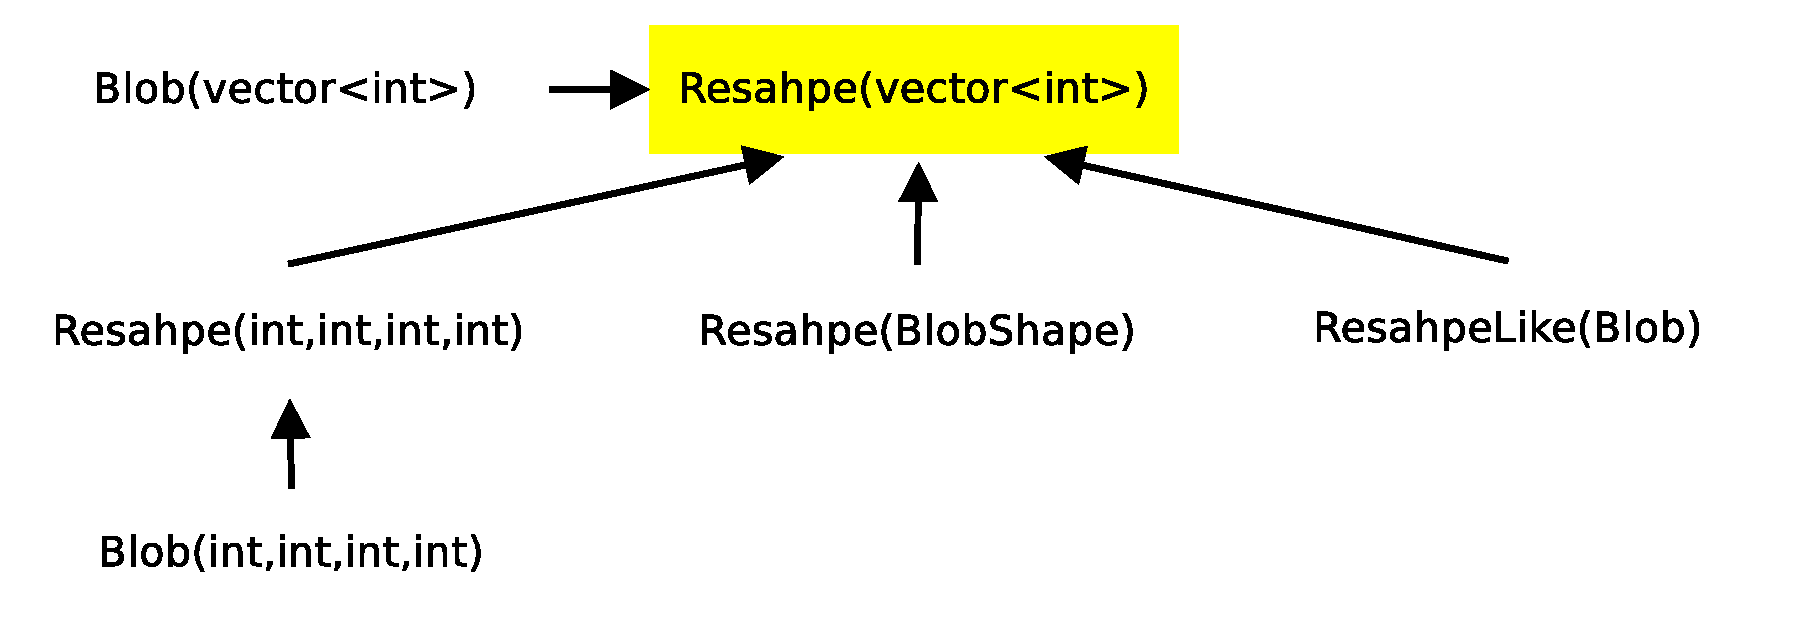
\includegraphics[height=5cm ,width=15cm,angle=0]{include/chp_blob_cls/figures/blob_architecture_reshape.eps}
\end{cnfigure}
% Section X.2.2
\subsection{数据指针的获取}
Blob中维护的数据包括data和diff两部分,内部的数据类型为SyncedMemory。Blob类通过成员函数来获取不同类型的数据指针,从而进行下一步的读取和写入操作。
\begin{cntable}{数据指针获取}{blob/architecture/getptr}
  \begin{tabular}{|l|l|l|l|}
    \hline
          & \makecell[cc]{\hei CPU} & \makecell[cc]{\hei GPU} & \\\hline
    \hei shape &  & gpu\_shape() &  \\ \hline
    \hei data  & \makecell[cl]{cpu\_data() \\ set\_cpu\_data() \\ mutable\_cpu\_data()} & gpu\_data() & shareData() \\ \hline
    \hei diff  & \makecell[cl]{cpu\_diff() \\ mutable\_cpu\_diff()} & \makecell[cl]{gpu\_diff() \\ mutable\_gpu\_diff()} & shareDiff() \\ \hline
  \end{tabular}
\end{cntable}
% Section X.2.3
\subsection{Blob中的数学运算}
Blob类中有一类函数涉及到代数运算操作,在Caffe中几乎所有运算相关操作都是通过内部调用cBLAS或cuBLAS运算库在CPU或GPU上完成的,这部份内容可以参考\ref{math/cpu/alg}和\ref{math/gpu/alg}。
\begin{cntable}{Blob中的数学运算}{blob/architecture/getptr}
  \begin{tabular}{|l|l|l|}
    \hline
    \makecell[cc]{\hei Blob类} & \makecell[cc]{\hei Caffe封装} & \makecell[cc]{\hei cBLAS或cuBLAS} \\ \hline
    Update() & caffe\_axpy() & \makecell[cl]{cblas\_*axpy \\ cublas*axpy} \\ \hline
    \makecell[cl]{asum\_data() \\ ausm\_diff()}  & \makecell[cl]{caffe\_cpu\_asum() \\ caffe\_gpu\_asum()} & \makecell[cl]{cblas\_*asum() \\ cublas*asum()} \\ \hline
    \makecell[cl]{sumsq\_data() \\ sumsq\_diff()}  & \makecell[cl]{caffe\_cpu\_dot() \\ caffe\_gpu\_dot()} & \makecell[cl]{cblas\_*dot() \\ cublas*dot()} \\ \hline
    \makecell[cl]{scale\_data() \\ scale\_diff()}  & \makecell[cl]{caffe\_scal() \\ caffe\_gpu\_scal()} & \makecell[cl]{cblas\_*scal() \\ cublas*scal()} \\ \hline
  \end{tabular}
\end{cntable}

% Section X.2.4
\subsection{BlobProto参数}
Blob类可以读入BlobProto对象中的数据,也可以将自身维护的数据保存到BlobProto对象中。
\begin{cnfigure}{BlobProto输入输出}{blob/architecture/blobproto}
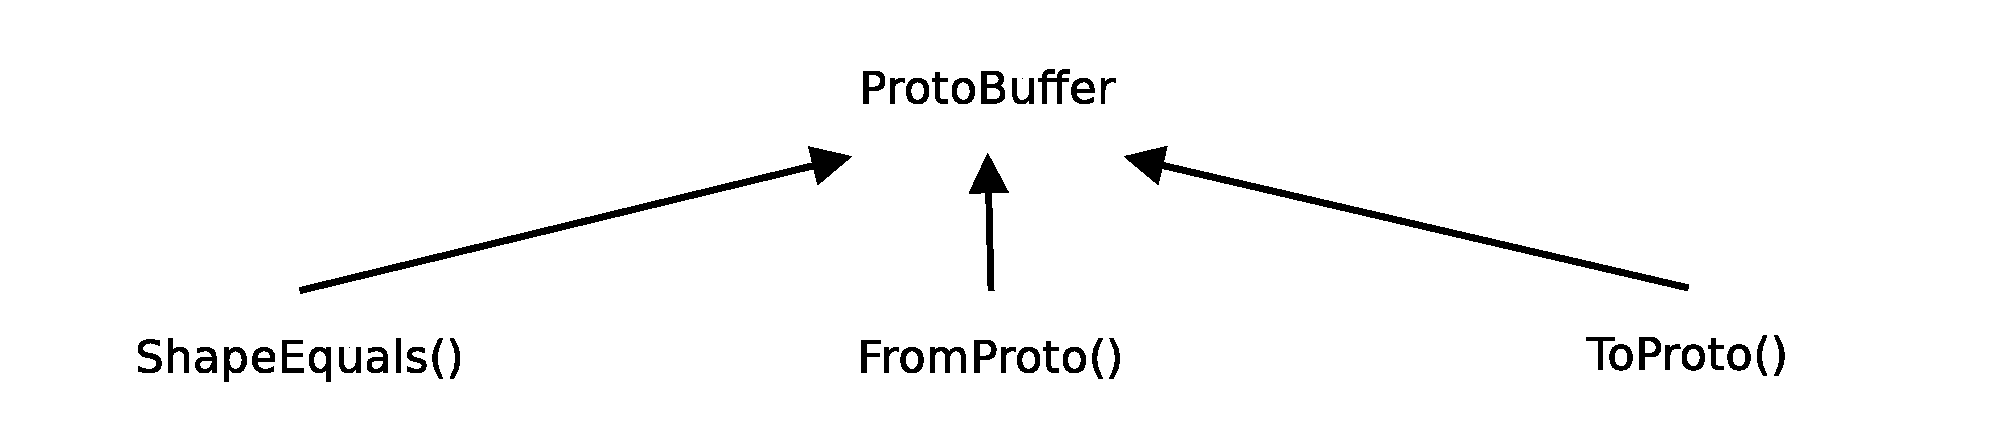
\includegraphics[height=3cm ,width=15cm,angle=0]{include/chp_blob_cls/figures/blob_architecture_proto.eps}
\end{cnfigure}
\chapter{网络定义Layer类}

\chapter{网络管理Net类}

\chapter{网络的运行Slover类}

%%%%%%%%%%%%%%%%%%%%%%%%%%

%%%%%%%%%%%%%%%%%%%%%%%%%
\cnbibliography{bibtex.bib}


% \appendix
\begin{cnappendix}
\chapter{编译指挥官Makefile}

\end{cnappendix}

\end{document}


%%% Local Variables:
%%% mode: latex
%%% TeX-master: 
%%% End:
